\documentclass[12pt, a4paper]{article}
\usepackage[utf8]{inputenc}
\usepackage[russian]{babel}
\usepackage[pdftex]{graphicx, color}
\usepackage{amsmath}
\usepackage{amsfonts}
\usepackage{amssymb}
\usepackage{amsthm}
\usepackage[left=2cm,right=1.5cm,top=1.5cm,bottom=2cm]{geometry}
\usepackage{indentfirst}
\usepackage{hyperref}

\usepackage{pbox}

\usepackage{setspace}
\onehalfspacing
\graphicspath{{pic/}}

\begin{document}

	\thispagestyle{empty}

	\begin{singlespace}
	\begin{titlepage}
		\begin{center}
			
\includegraphics[height = 3cm]{msu.png}

			{\scshape Московский государственный университет имени М.~В.~Ломоносова}\\
			Факультет вычислительной математики и кибернетики\\
			\centerline{\hfill\hrulefill\hrulefill\hrulefill\hrulefill\hfill}

			\vfill

			{\LARGE Отчет к шестому заданию практикума на ЭВМ: \\ Использование Cython для решения задачи кластеризации}

			\vspace{1cm}

		\end{center}

		\vfill
		\begin{flushright}
			\textit{Студент 3 курса ВМК (317 группа):}\\
				Оспанов А.М.

			\vspace{5mm}

		\end{flushright}

		\vfill

		\begin{center}
		Москва, 2015
		\end{center}
	\end{titlepage}
	\end{singlespace}

	\tableofcontents


	\newpage
	\section{Введение}
		Данный отчет написан к шестому заданию практикума на ЭВМ 317 группы. Тема задания: Использование Cython для решения задачи кластеризации. Отчет написан студентом 317 группы -- Оспановым Аятом.

		В данной работе были реализованы алгоритмы кластеризаций k-Means и k-Medoids на языках Python, Cython и C++. Были проведены исследования по производительности кодов на разных языках и их точности на городах Мира. Также результаты были визуализированы.

	\newpage
	\section{Основная часть}
		\subsection{Математические выкладки}
			Для кластеризации городов на сфере, нужно найти расстояние по сфере. Это расстояние высчитывается через следующую формулу:

			$$L = R * arccos(sin(\theta_1) * sin(\theta_2) + cos(\theta_1) * cos(\theta_2) * cos(\varphi_1 - \varphi_2))$$
			где $\theta_1, \theta_2$ - широты городов, $\varphi_1, \varphi_2$ - долготы городов.

			Для нахождения центров масс использовался поворот относительно векторного произведения. Сперва точки переводились в трехмерное пространство через следующие формулы:
			\begin{align*}
			x &= r * cos(\theta) * cos(\varphi) \\
			y &= r * cos(\theta) * sin(\varphi) \\
			z &= r * sin(\theta)
			\end{align*}

			Далее находилось их векторное произведение и нормировалось. Затем относительно этой оси первый вектор поварачивался на угол умноженный на его вес, поделенный на сумму весов двух векторов. Угол высчитывался с помощью скалярного произведения. Далее найденная точка переводилась в сферическую систему.
			

		\newpage
		\subsection{Замер производительности}
		\label{sssec:comp}
			Для замера производительности ставилось точное количество итераций, равное 50. Т.е. алгоритм не выходил раньше 50 итераций, даже если сходился. После замеров, получились следующие результаты:

			\begin{center}
			\begin{tabular}{c c}
				k-Means на Python & k-Medoids на Python \\

				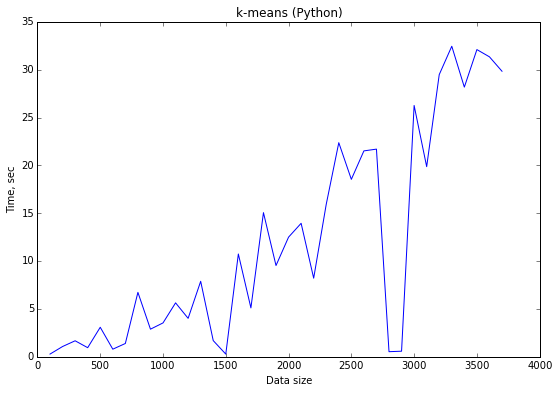
\includegraphics[width=8cm]{python_kmeans_time.png} &
				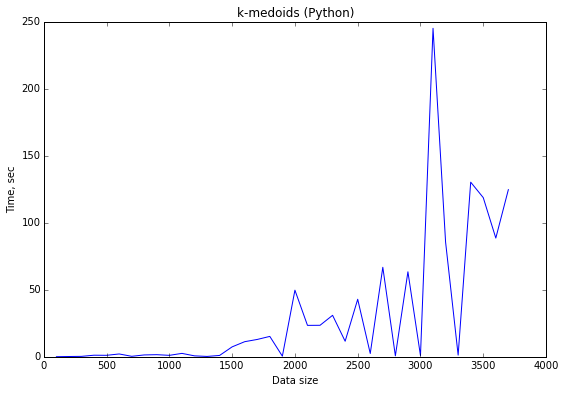
\includegraphics[width=8cm]{python_kmedoids_time.png} \\

				k-Means на Cython & k-Medoids на C++ \\

				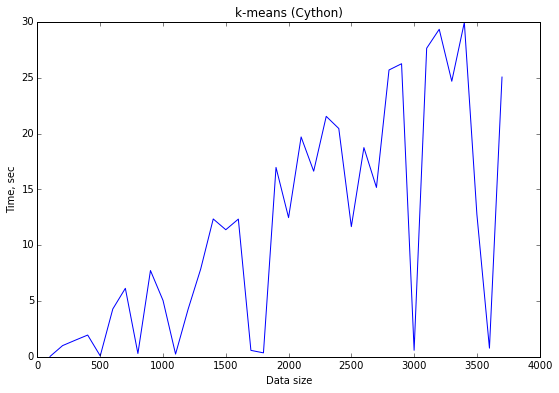
\includegraphics[width=8cm]{cython_kmeans_time.png} &
				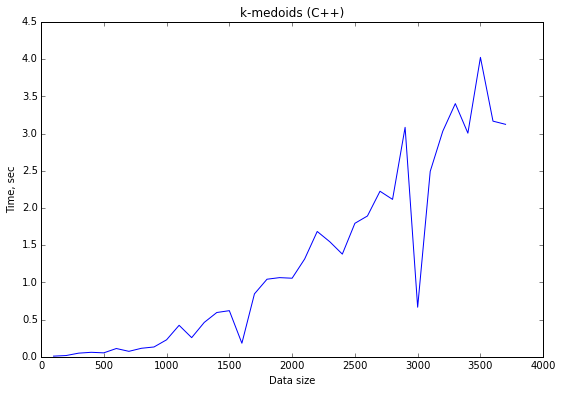
\includegraphics[width=8cm]{cpp_kmedoids_time.png} \\
			\end{tabular}
			\end{center}

			Из таблиц видно, что k-Means работает за время $O(N)$, а k-Medoids за $O(N^2)$, где N - количество данных. Это подтверждается теорией, т.к. k-Means вычисляет расстояние до центров масс, а k-Medoids вычисляет расстояния от каждой точки до каждой точки в кластере.

			\begin{center}
			\begin{tabular}{c c}
				Сравнение скоростей k-Means &
				Сравнение скоростей k-Medoids \\

				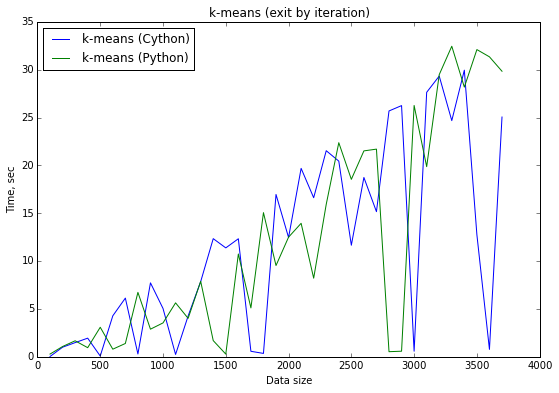
\includegraphics[width=8cm]{python_vs_cython_k_means.png} &
				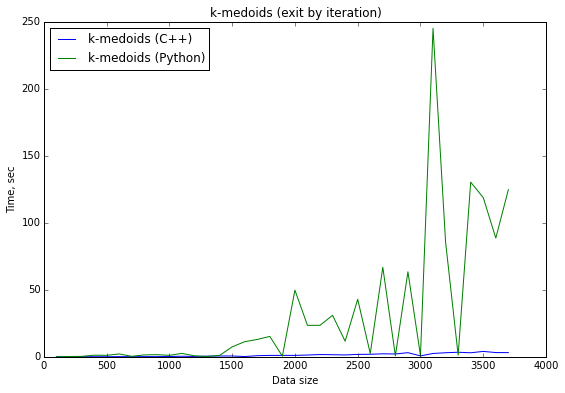
\includegraphics[width=8cm]{python_vs_cpp_k_medoids.png} \\
			\end{tabular}
			\end{center}

			Как видно из таблицы, реализации k-Means на Python и Cython почти одинаковые, но в следующей таблице (по аппроксимации) можно увидеть, что реализация на Cython ускоряется по сравнению с реализацией на Python, следовательно для дальнейших тестов выберем именно реализацию на Cython. Реализации k-Medoids на Python и C++ отличаются в несколько десятков раз. Из следующей таблицы можно увидеть, что реализация на C++ ускоряется очень быстро, по сранению с реализацией на Python. Тут без сомнений выбирается реализация на C++.

			\begin{center}
			\begin{tabular}{c c}
				\pbox{8cm}{Относительная скорость \\ Python к Cython в k-Means} &
				\pbox{8cm}{Относительная скорость \\ Python к C++ в k-Medoids} \\

				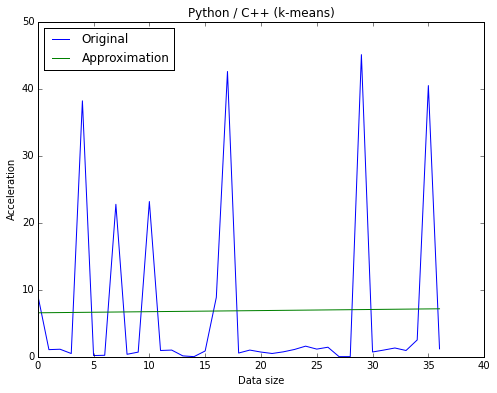
\includegraphics[width=8cm]{python_by_cpp_kmeans.png} &
				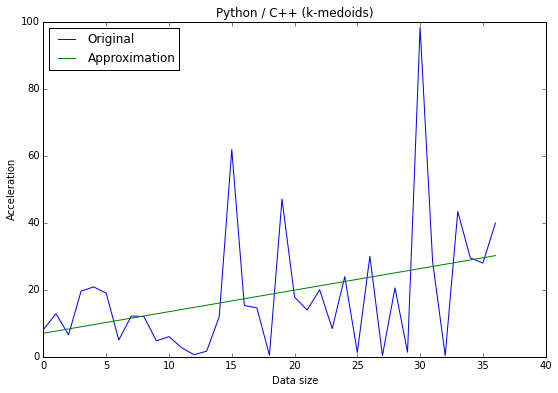
\includegraphics[width=8cm]{python_by_cpp_kmedoids.png} \\
			\end{tabular}
			\end{center}

			Далее для интереса приведем сранительную таблицу всех методов
			\begin{center}
				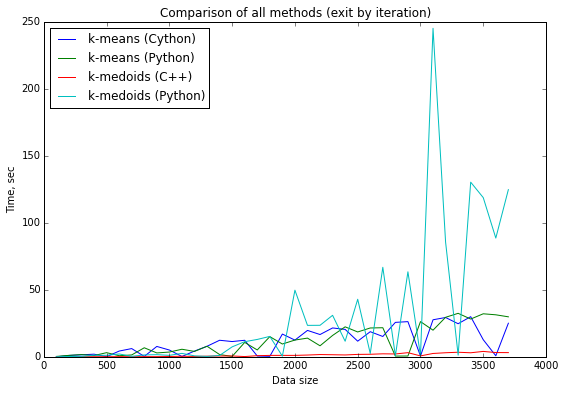
\includegraphics[width=10cm]{python_all_comparison.png}
			\end{center}


		\newpage
		\subsection{Тестирование алгоритмов}
		\label{sssec:test}
			Для дальнейших исследований алгоритм был настроен на выход по схождению.
			Приведем таблицу точностей для методов во всех регионах:

			\begin{center}
			\begin{tabular}{| l | l | l | l | l | l | l | l |}
			\hline
			& Мир & Африка & Азия & Австралия & Европа & С. Америка & Ю. Америка \\
			\hline
			k-Means & 0.4115 & 0.4055 & 0.5484 & 0.5517 & 0.2607 & 0.3652 & 0.4403 \\
			\hline
			k-Medoids & 0.4928 & 0.3947 & 0.5760 & 0.2675 & 0.4062 & 0.0970 & 0.3524 \\
			\hline
			\end{tabular}
			\end{center}

			Далее приведем результаты работ алгоритмов (изображения векторные):
			\begin{center}
			\begin{tabular}{l r}
				k-Means & k-Medoids \\
			\end{tabular}

			Африка

			\begin{tabular}{c c}
				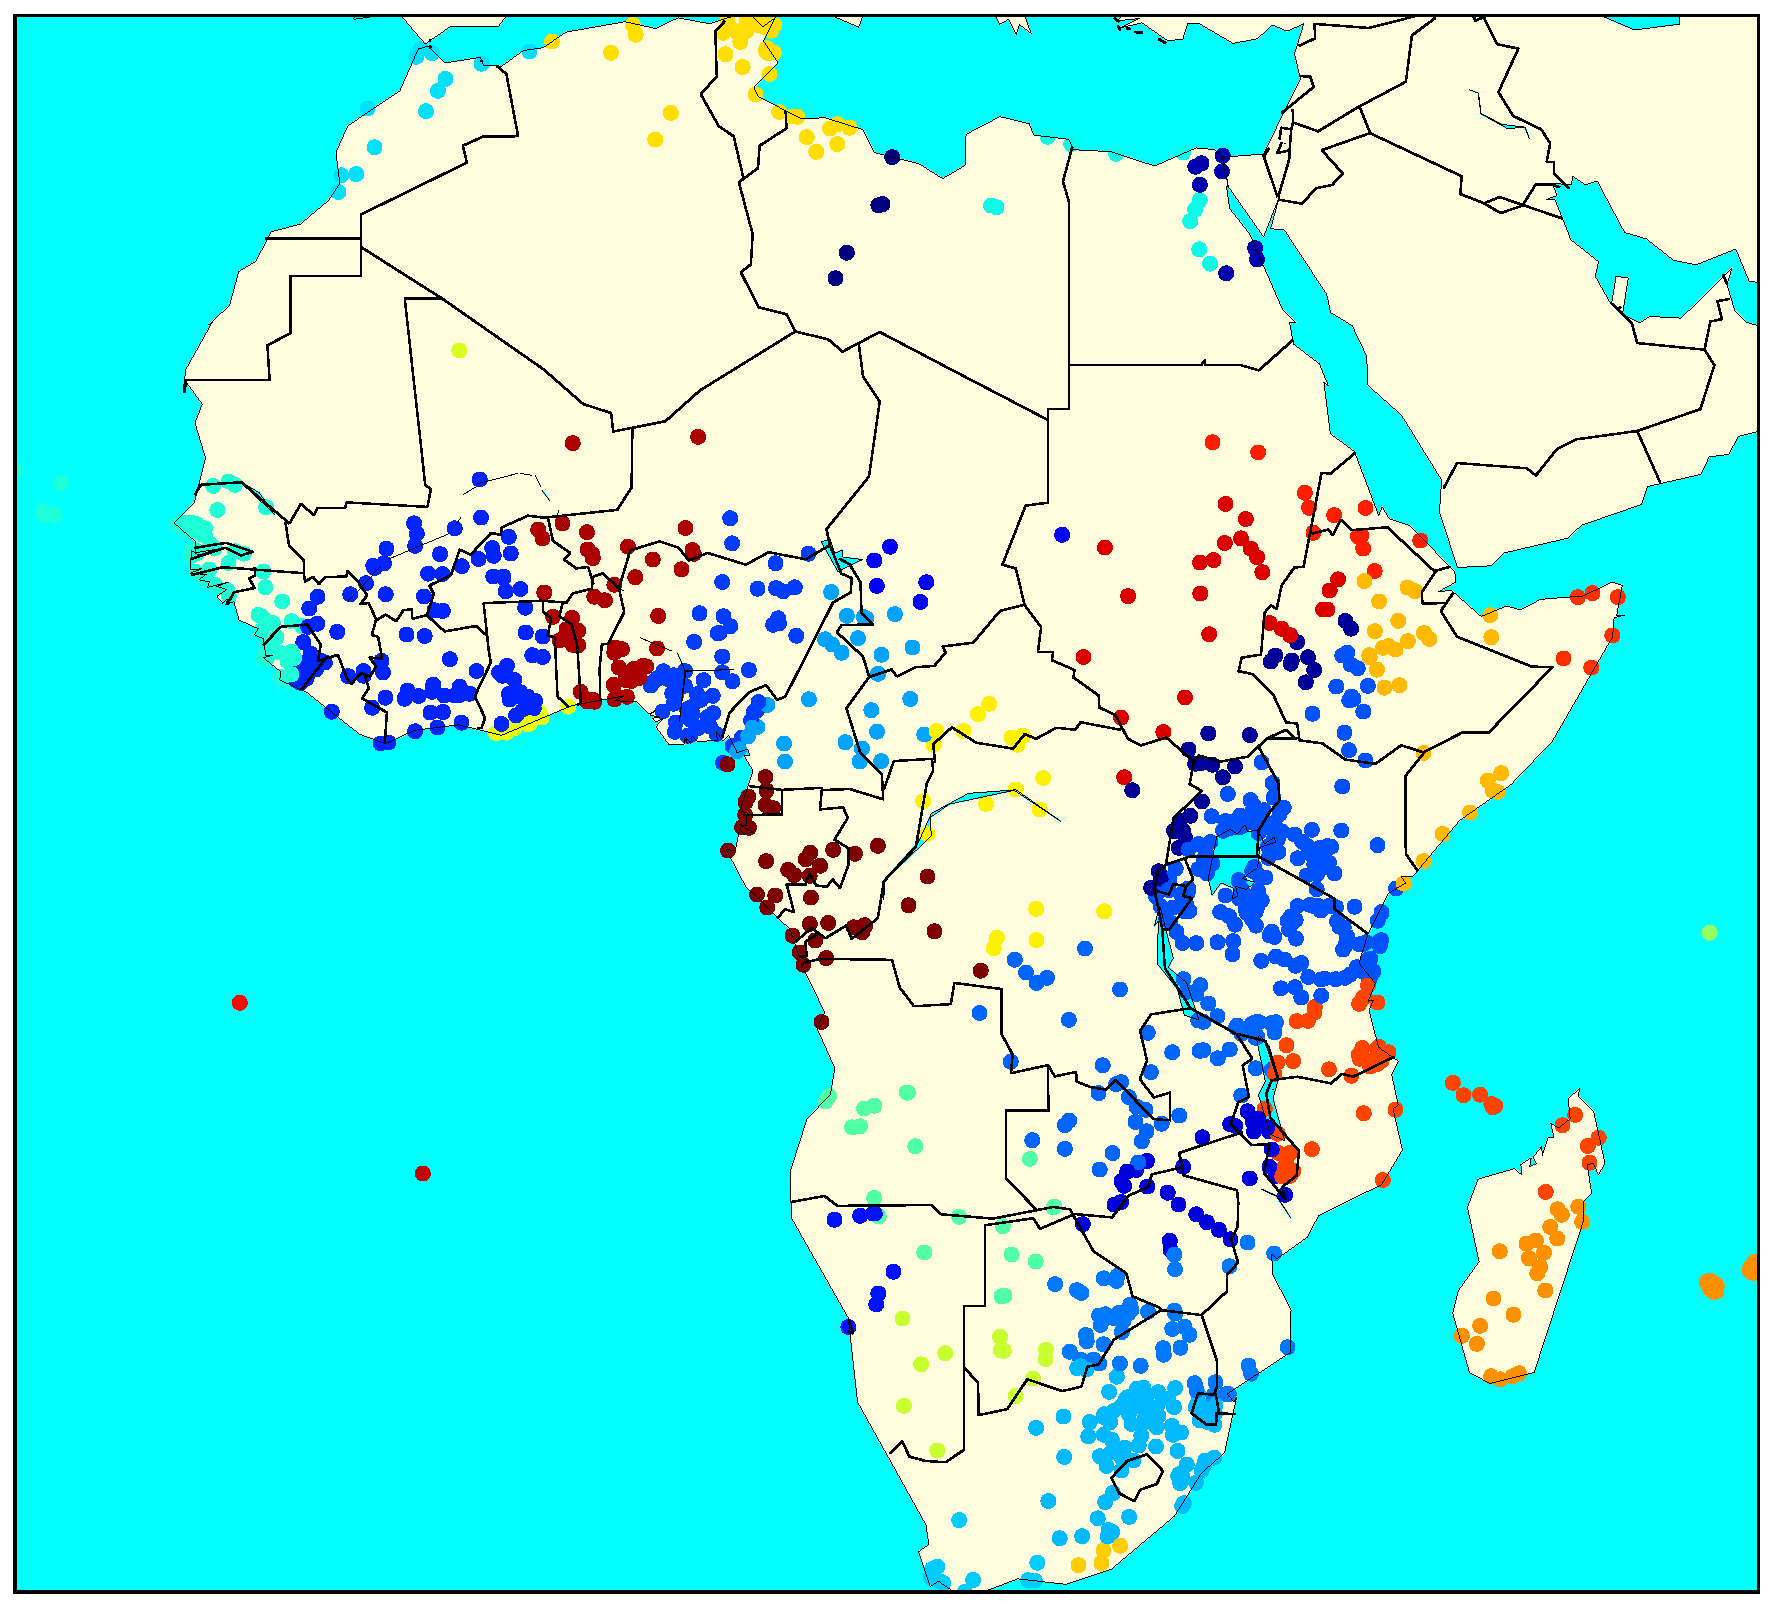
\includegraphics[width=8cm]{AF_k_means.pdf} &
				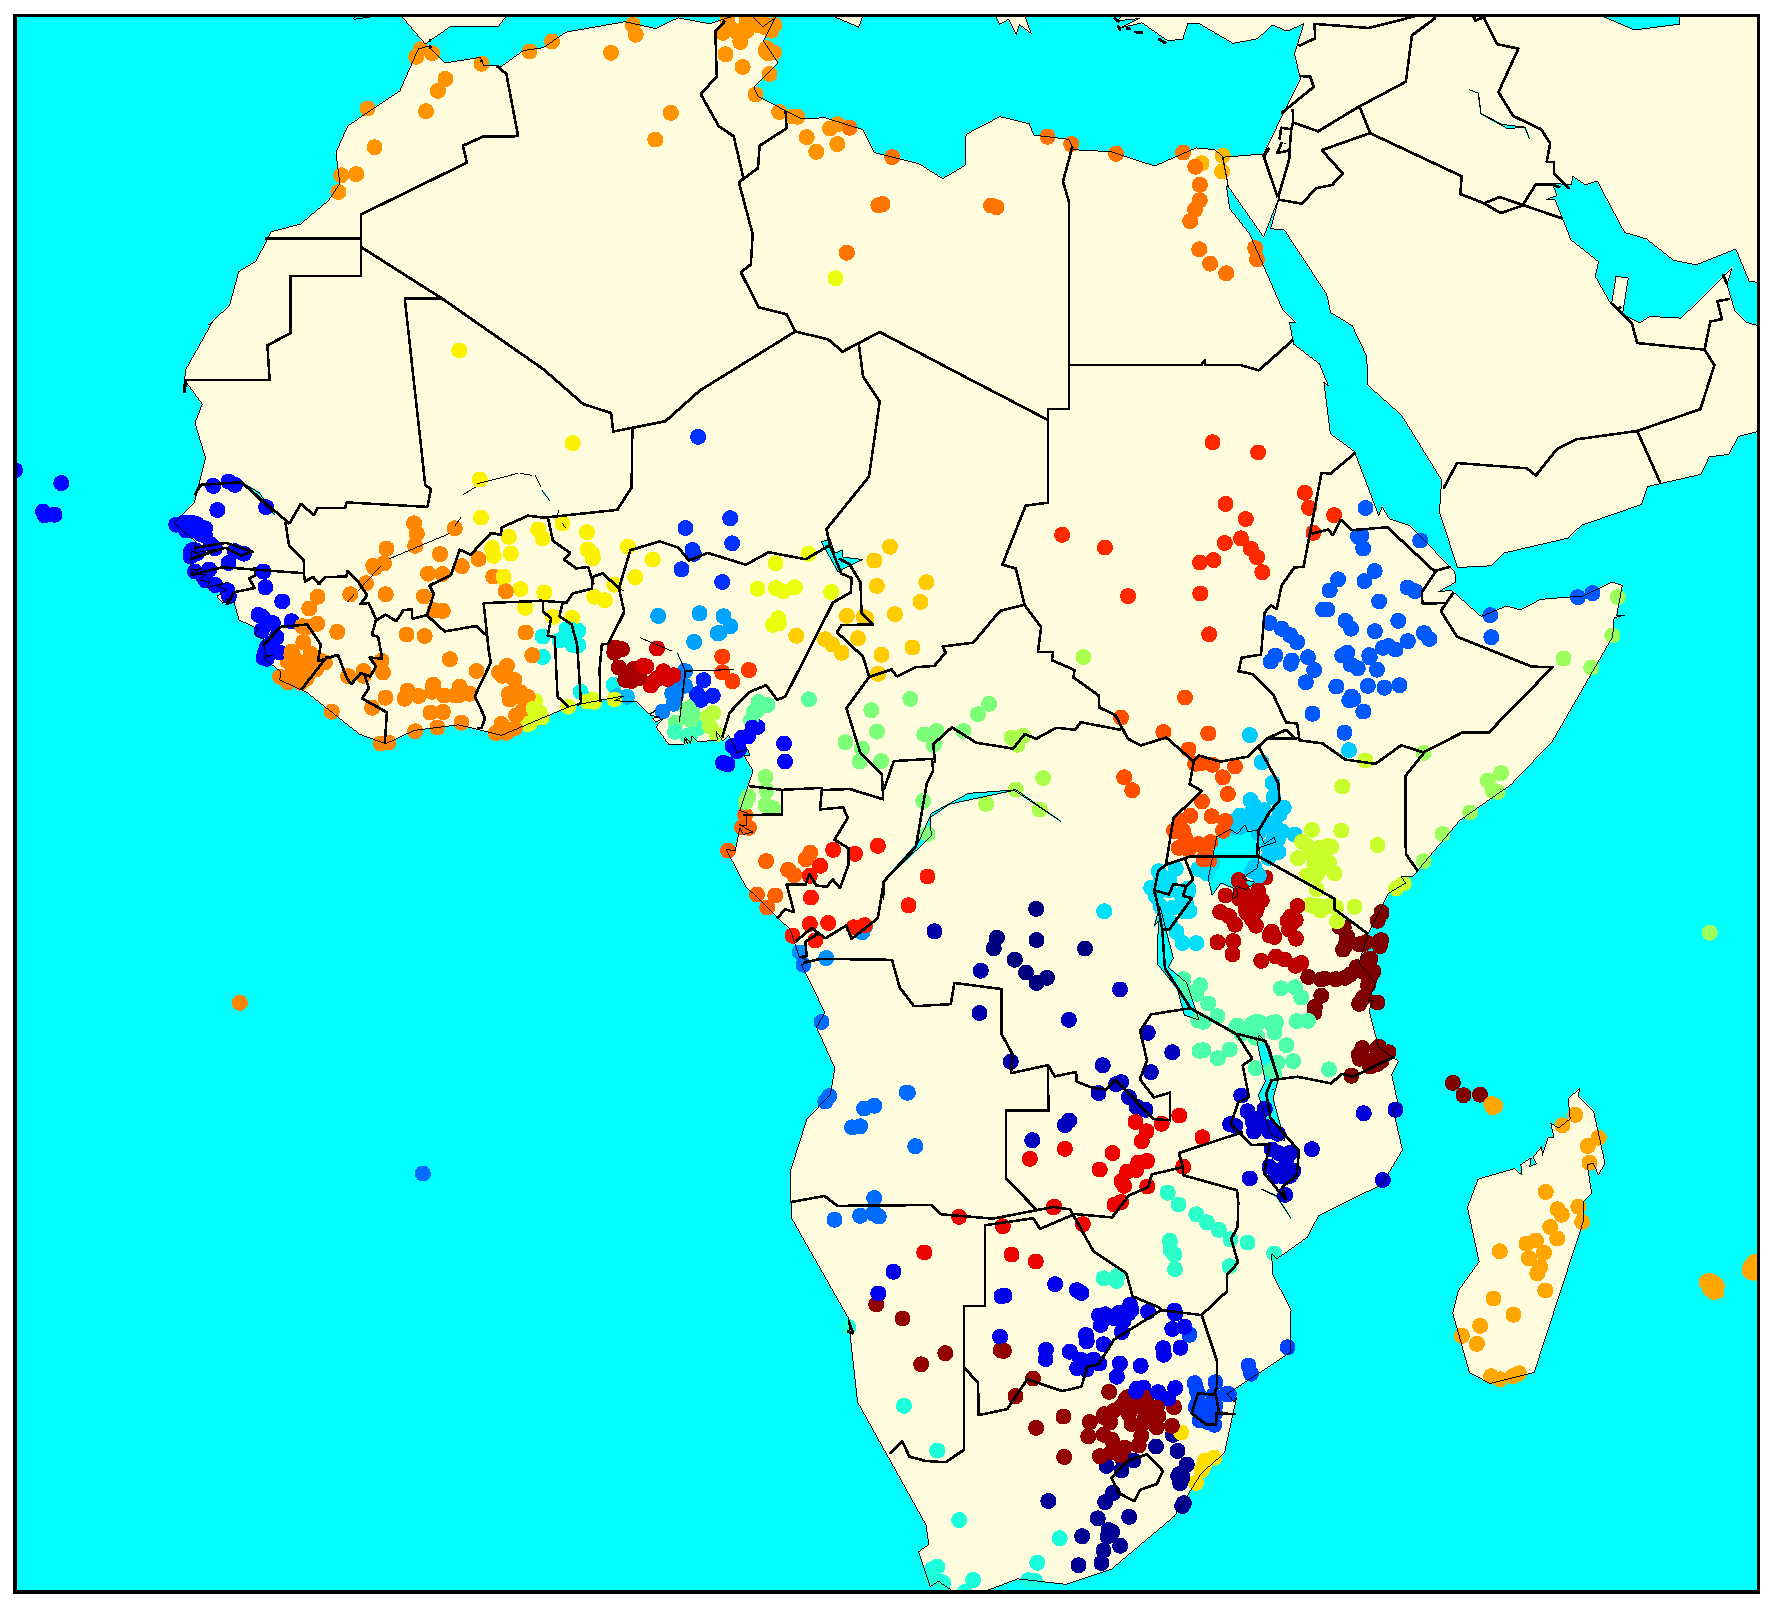
\includegraphics[width=8cm]{AF_k_medoids.pdf} \\
			\end{tabular}

			Азия

			\begin{tabular}{c c}
				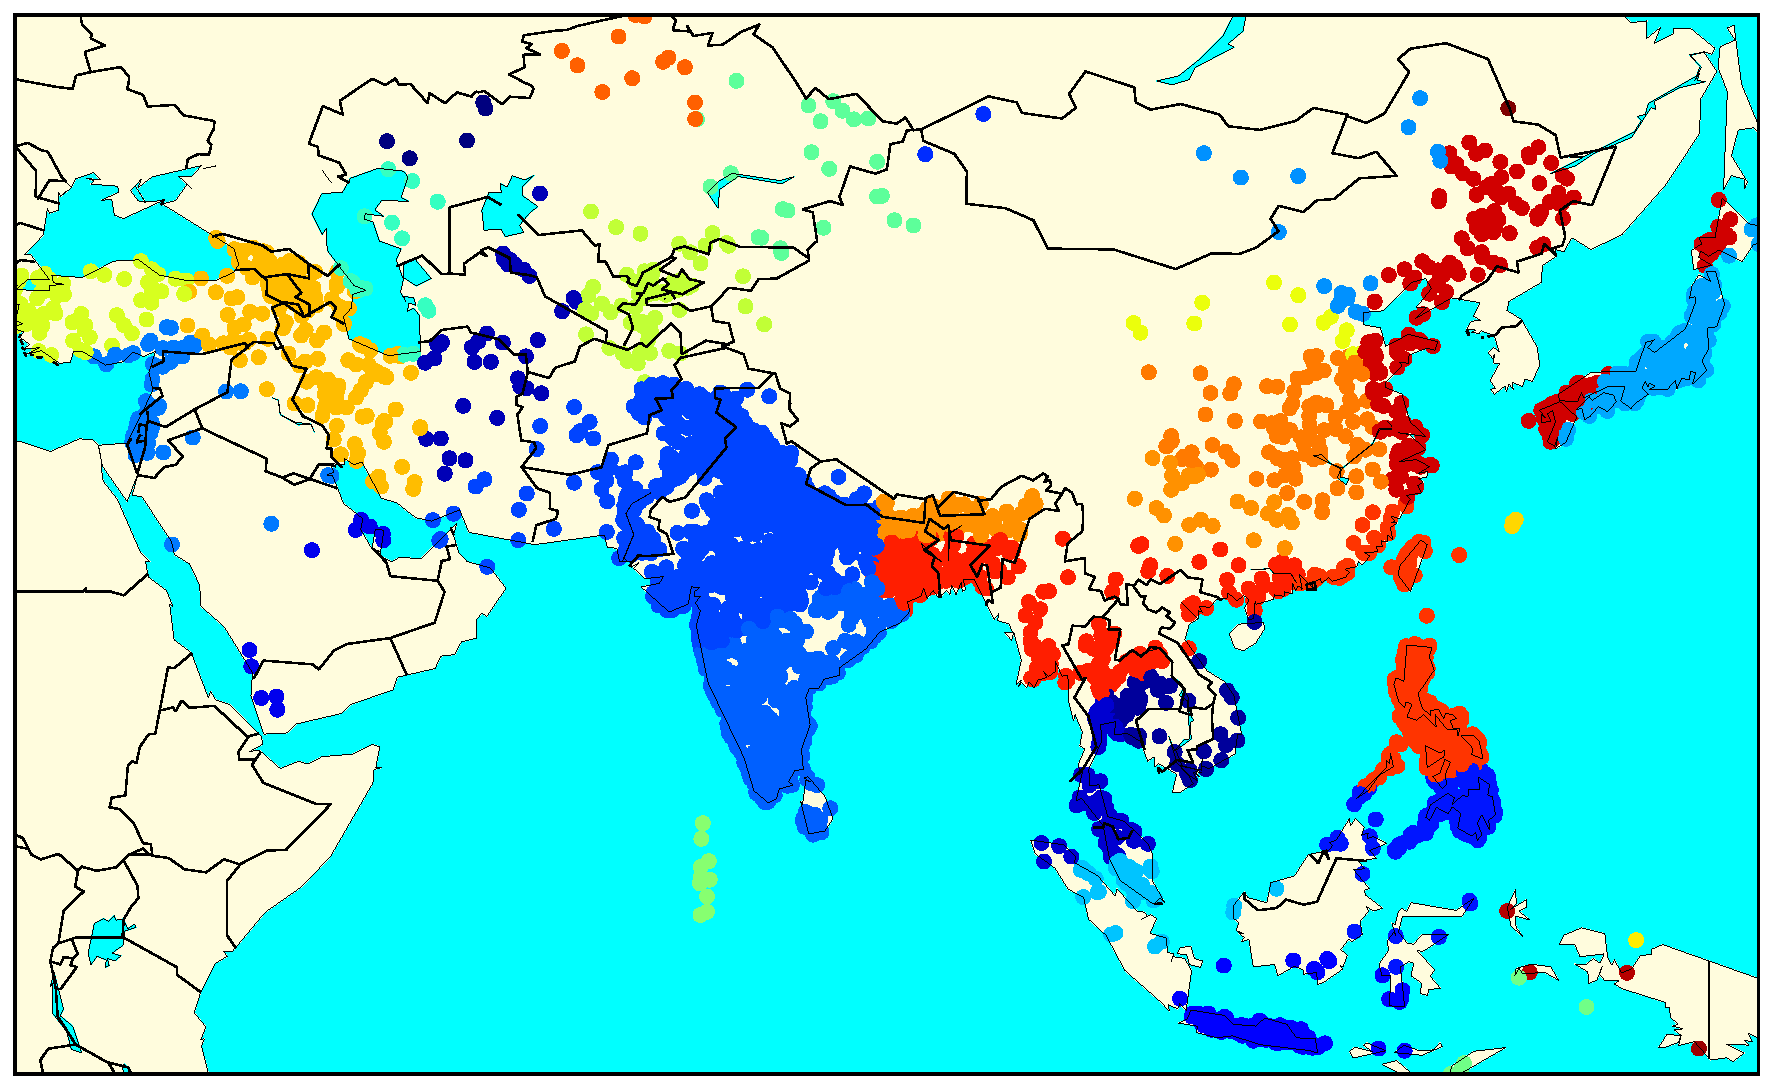
\includegraphics[width=8cm]{AS_k_means.pdf} &
				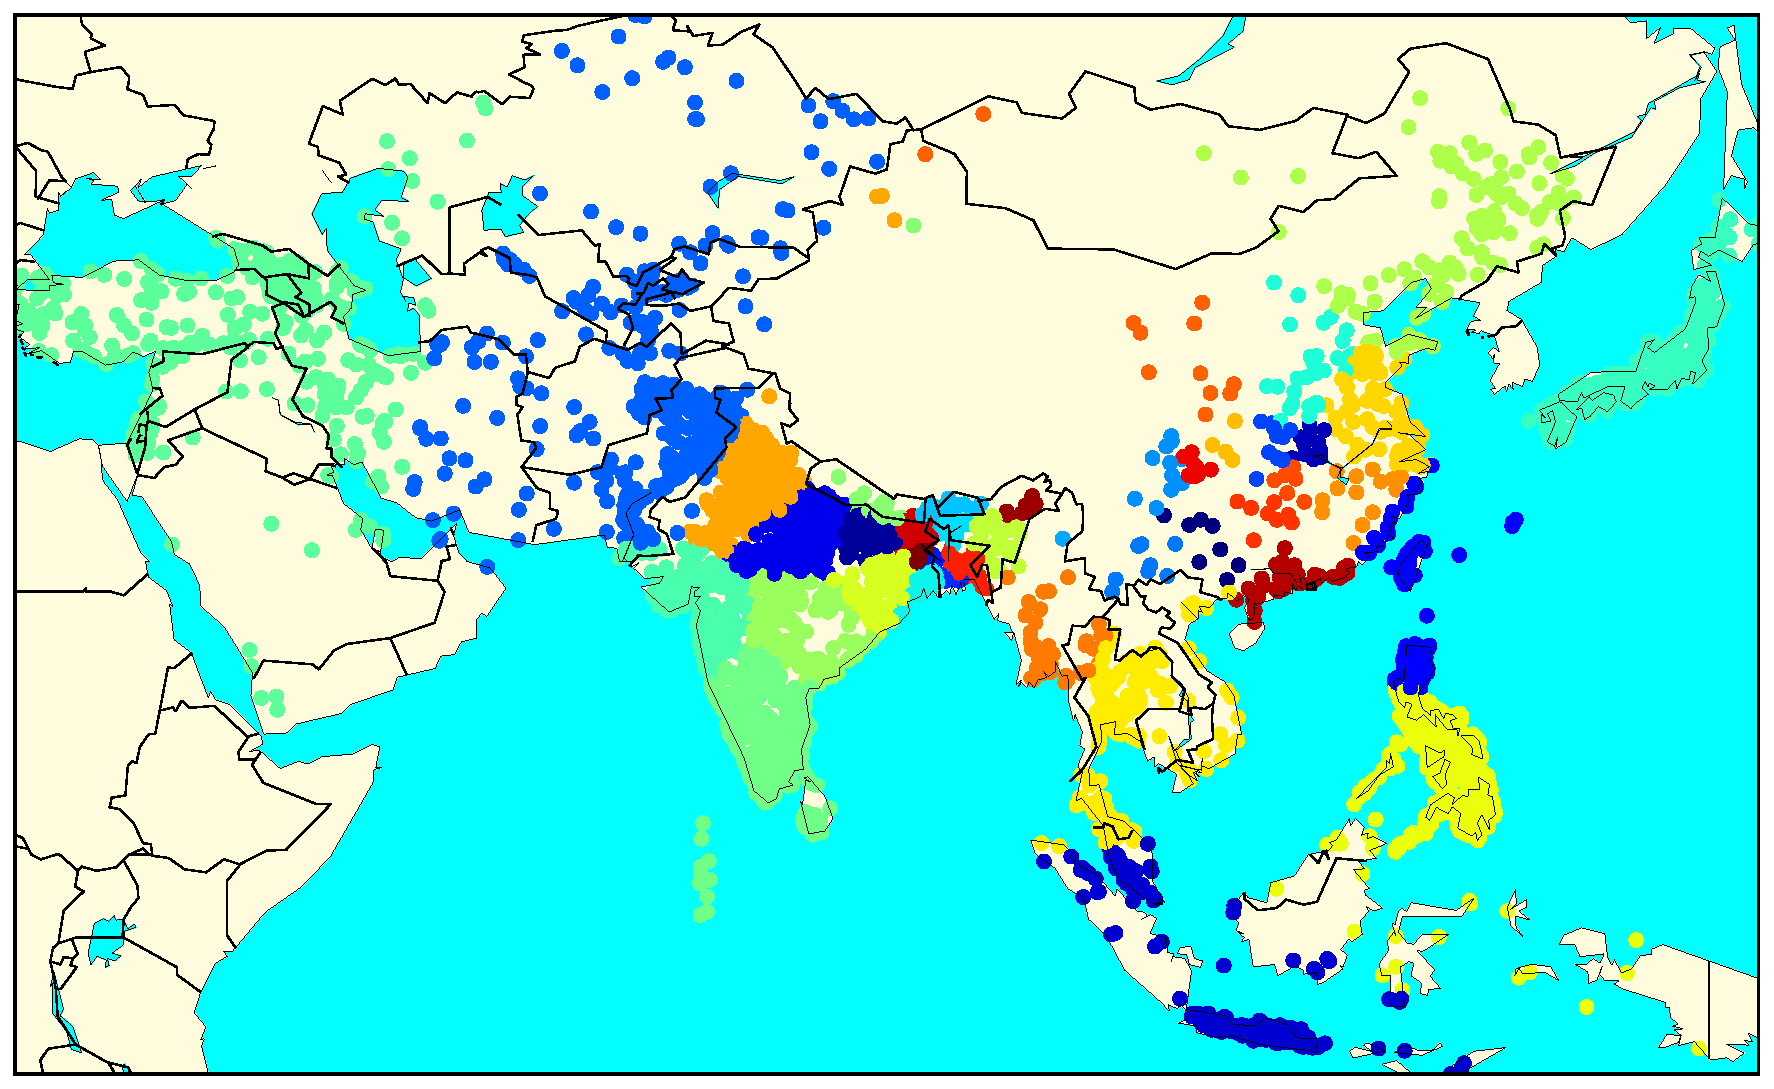
\includegraphics[width=8cm]{AS_k_medoids.pdf} \\
			\end{tabular}

			Австралия

			\begin{tabular}{c c}
				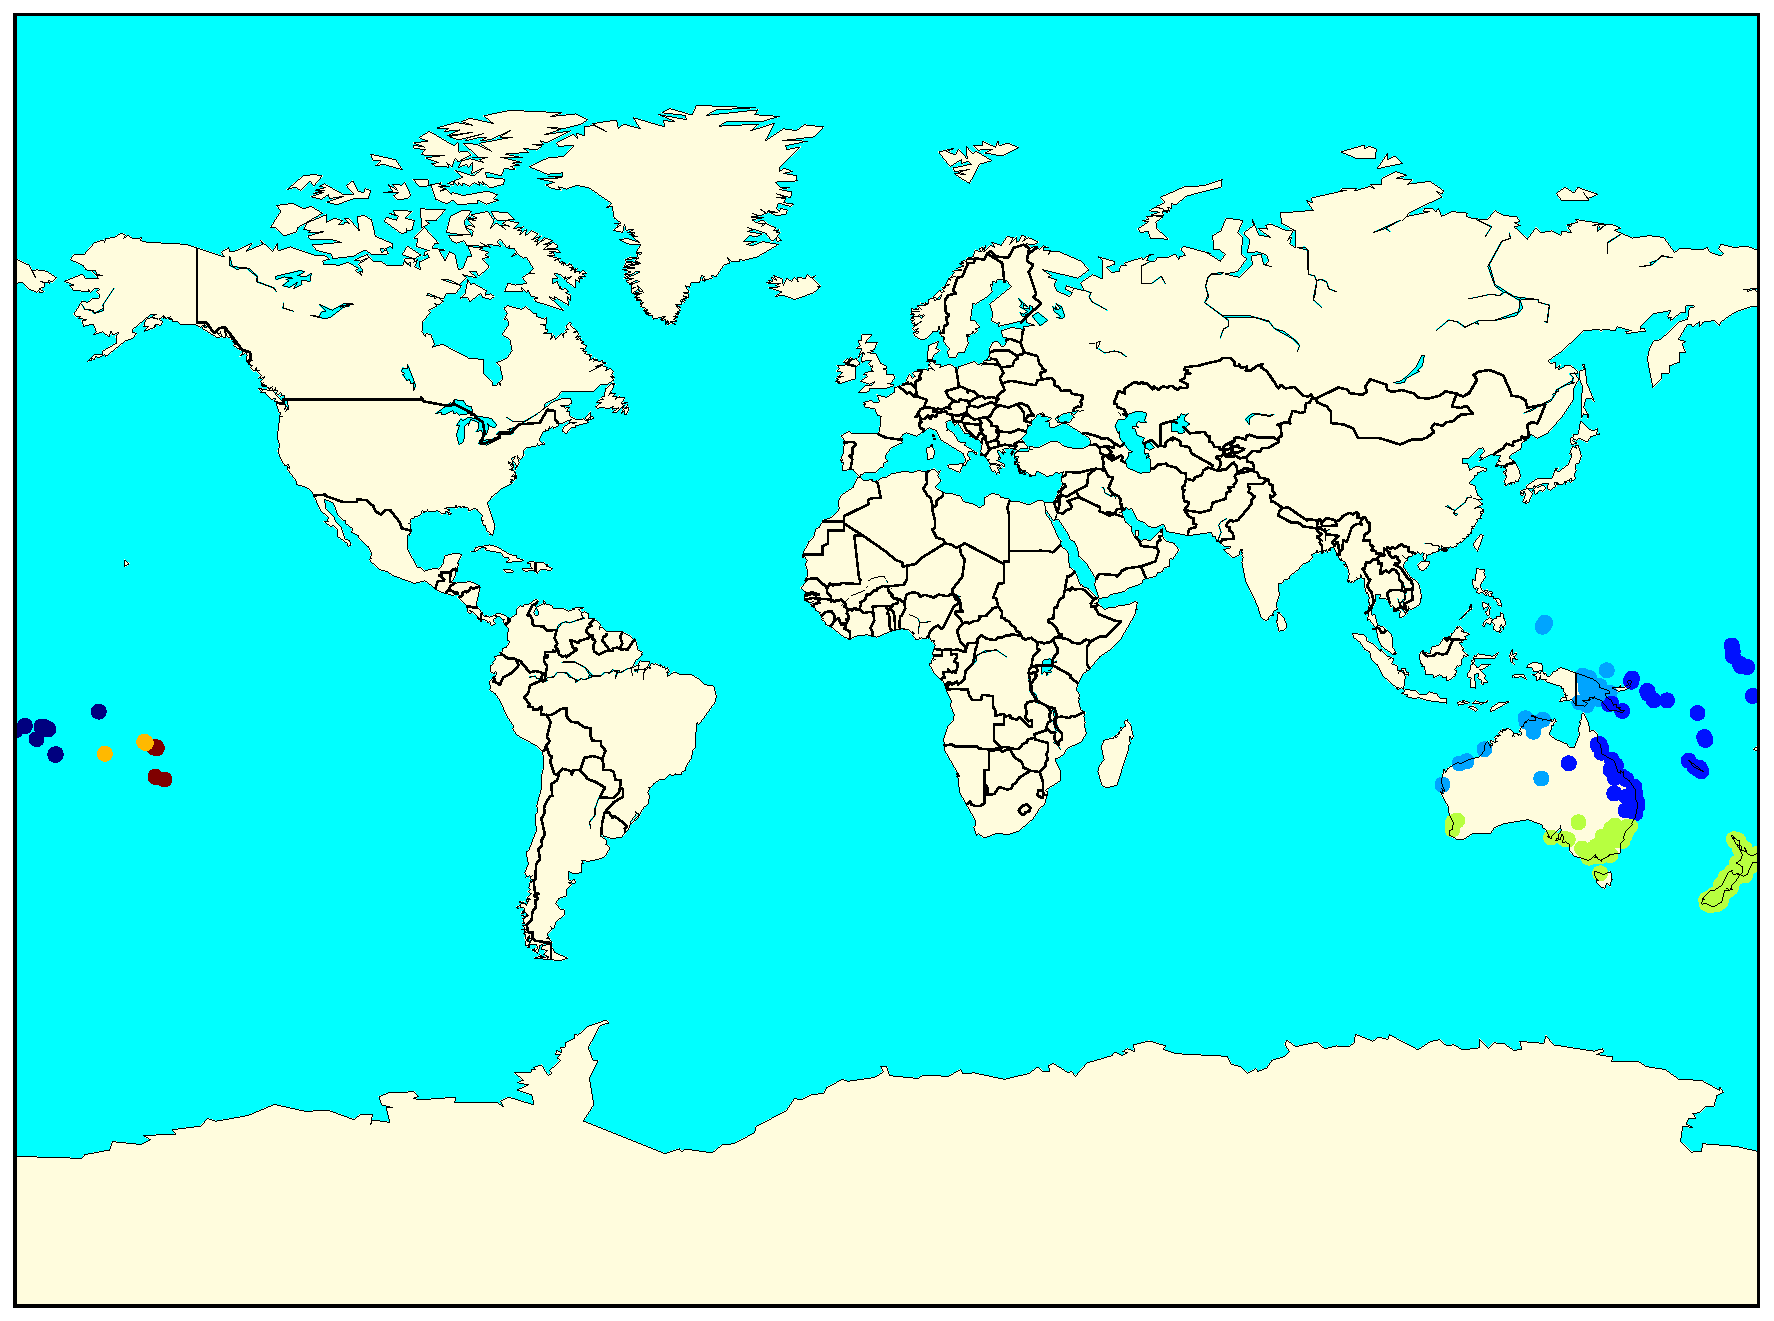
\includegraphics[width=8cm]{OC_k_means.pdf} &
				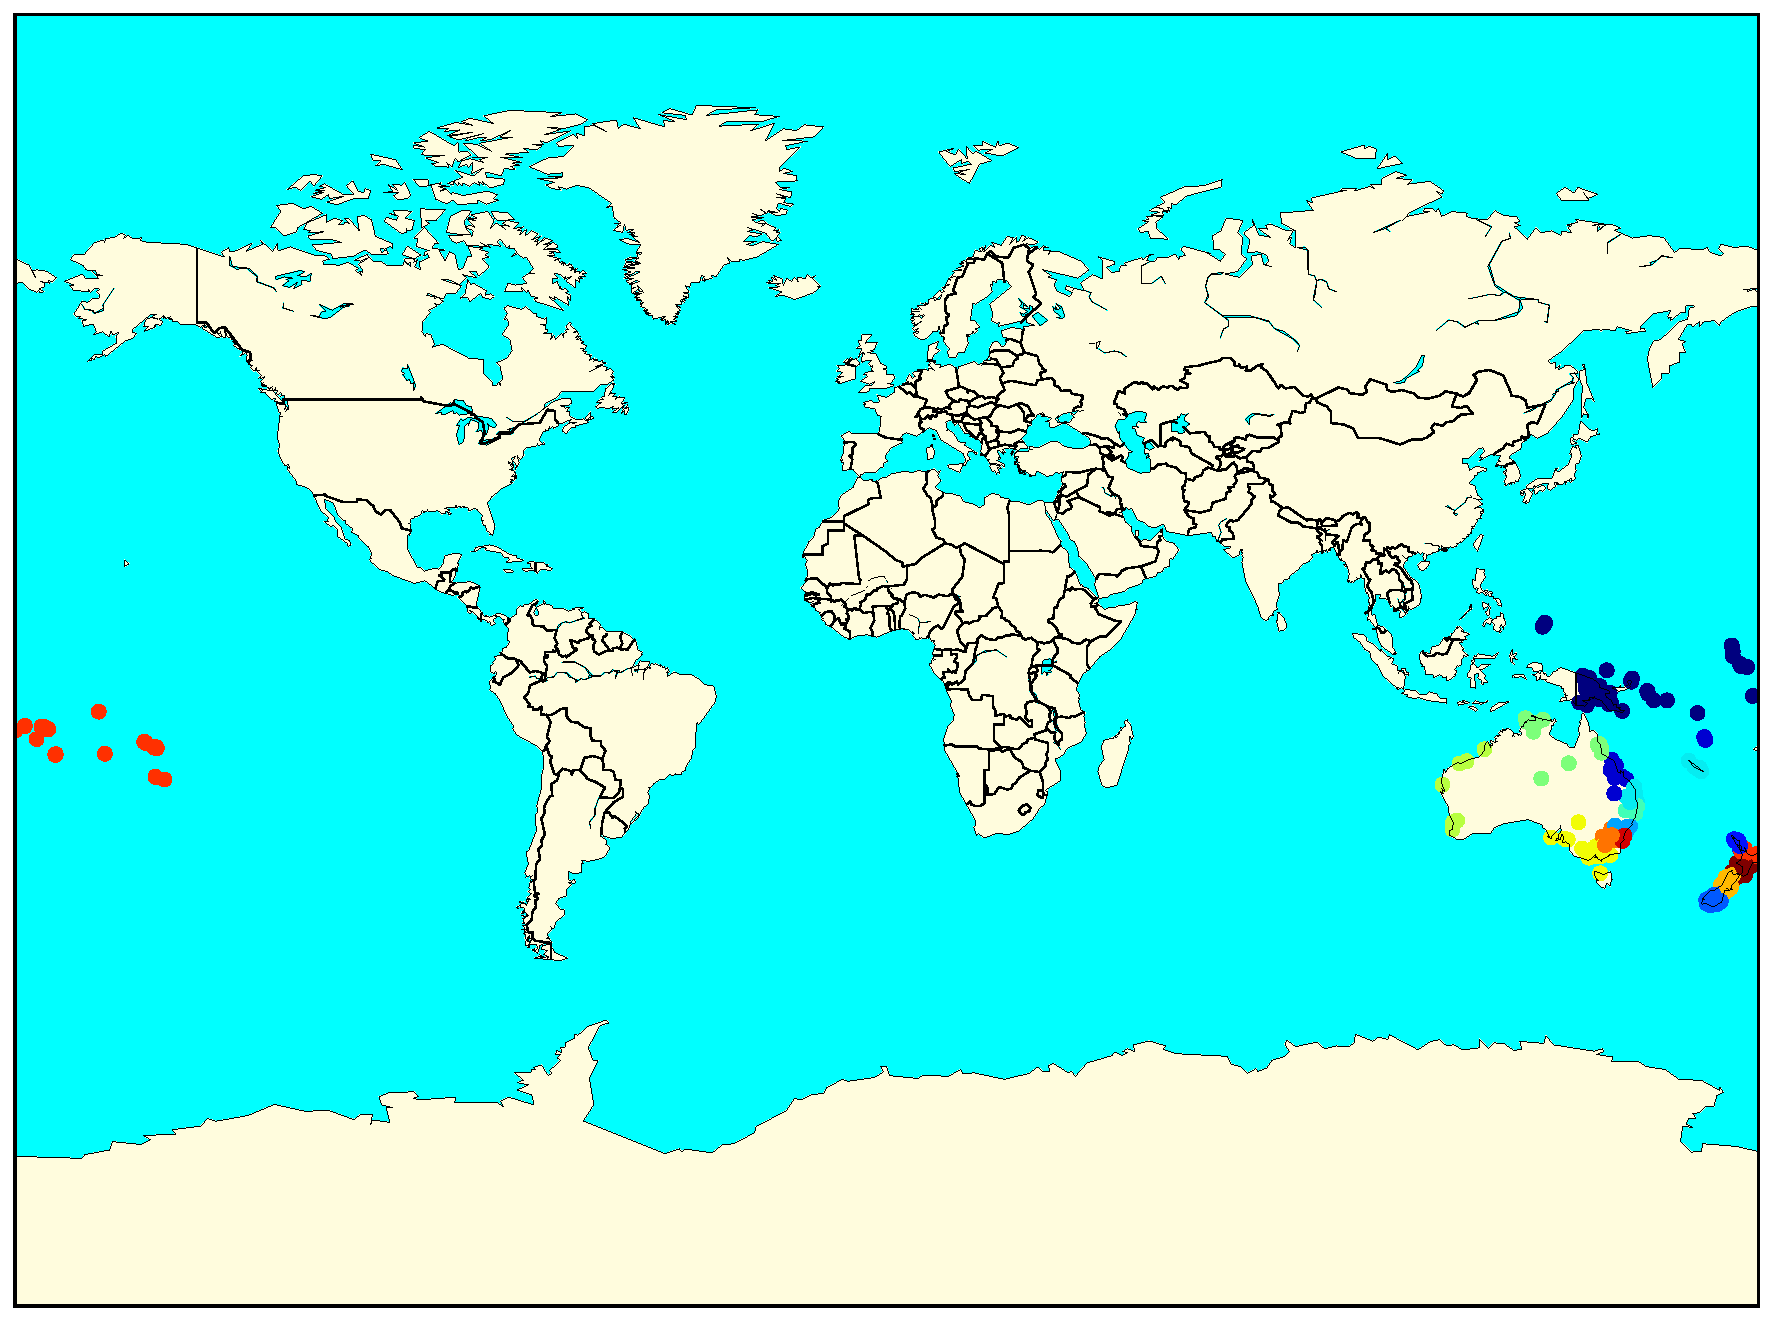
\includegraphics[width=8cm]{OC_k_medoids.pdf} \\
			\end{tabular}

			Европа

			\begin{tabular}{c c}
				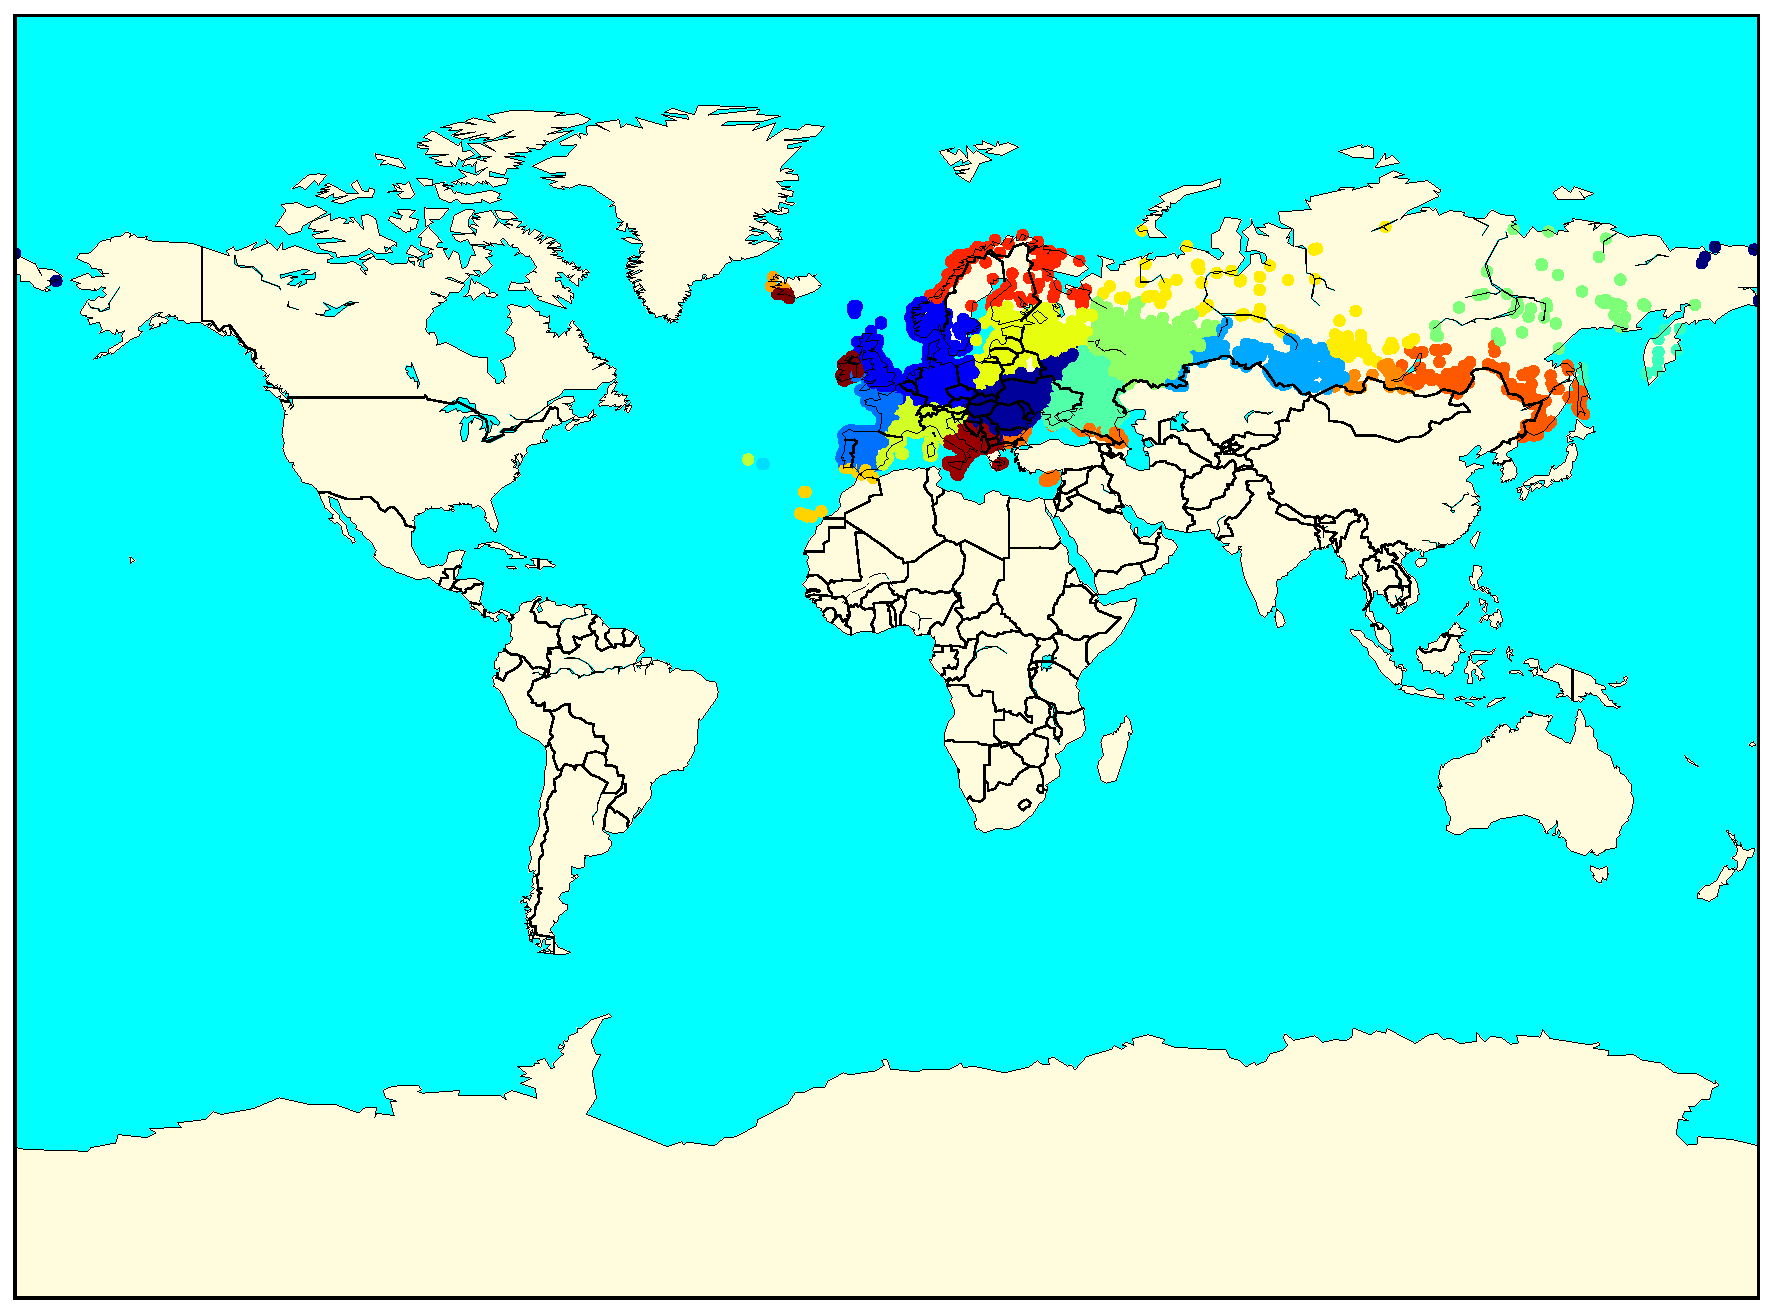
\includegraphics[width=8cm]{EU_k_means.pdf} &
				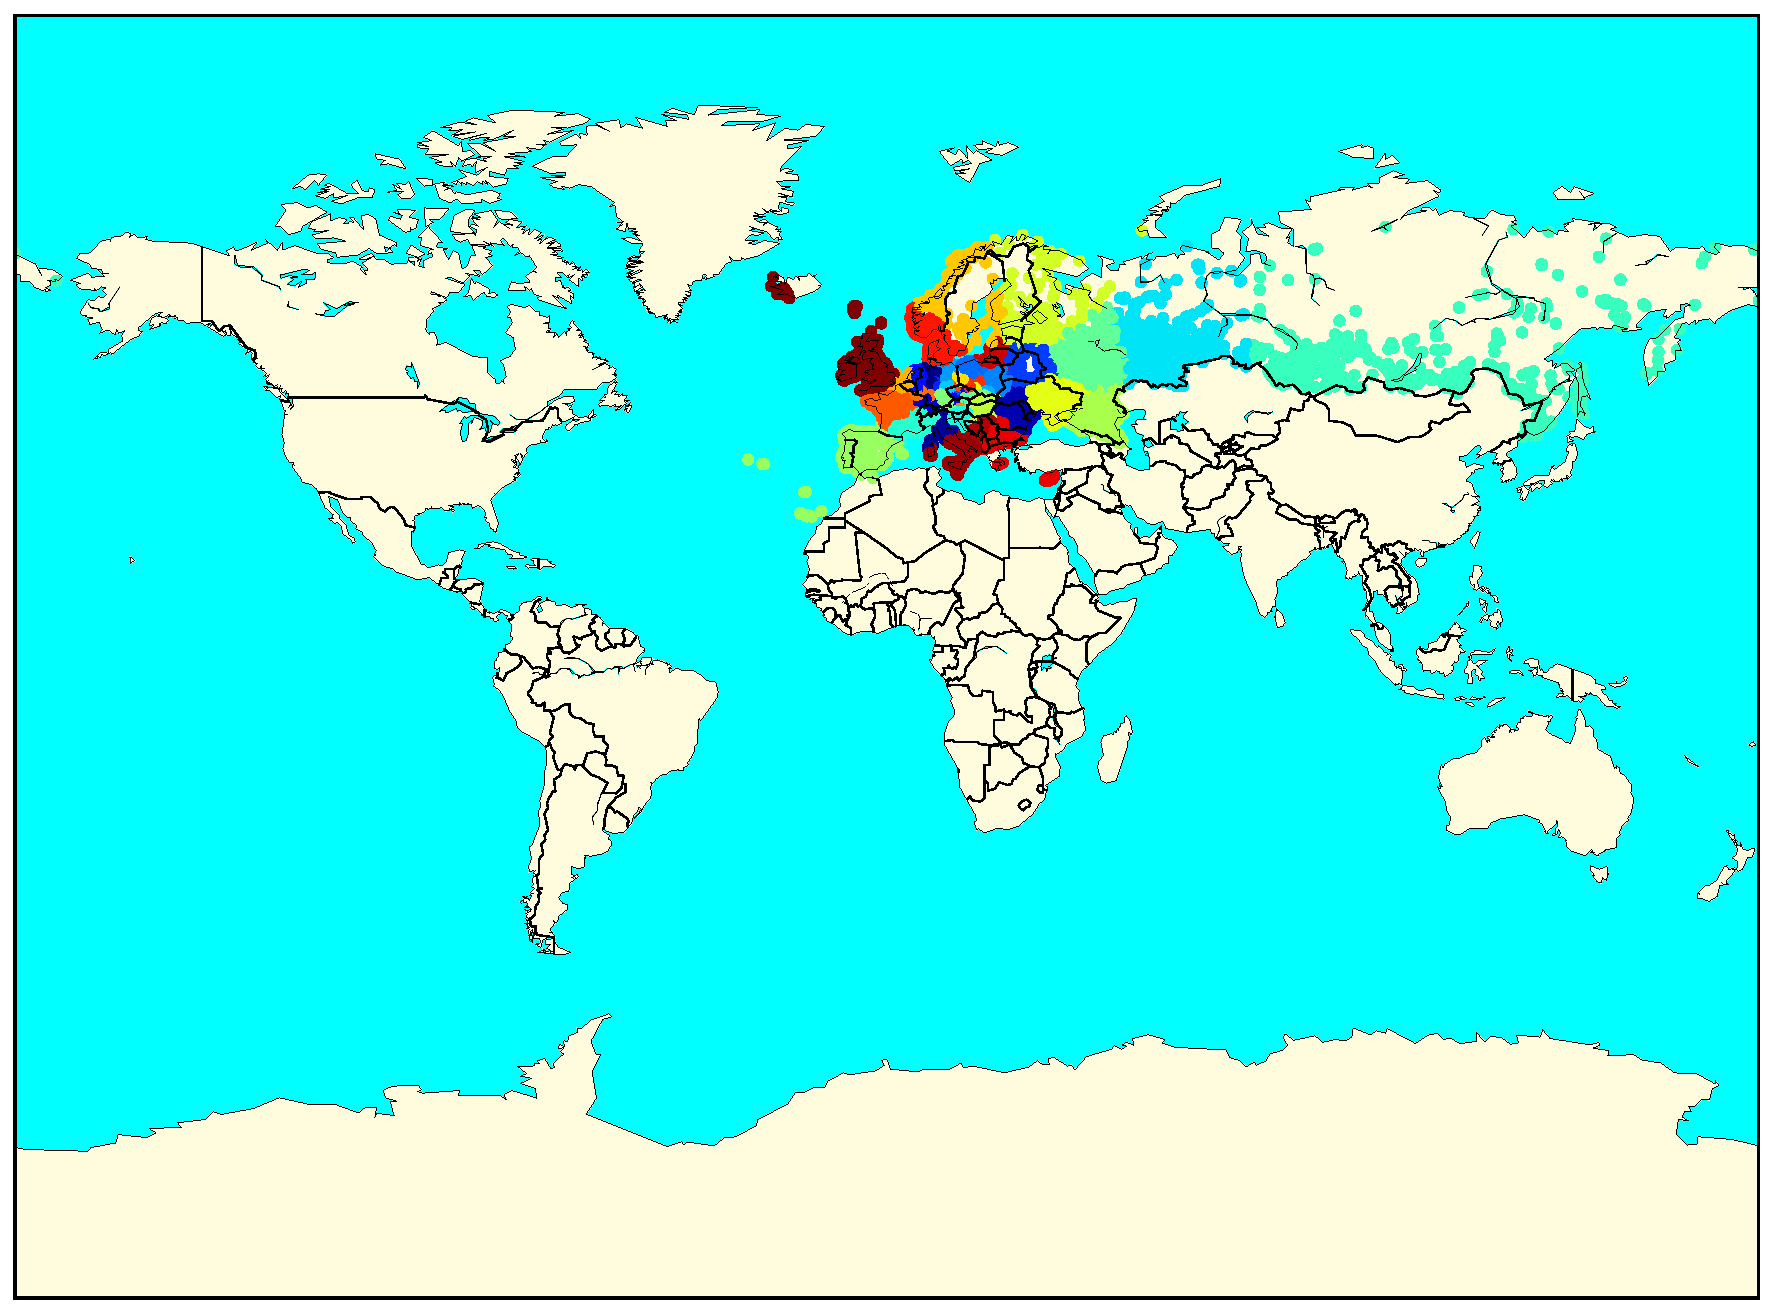
\includegraphics[width=8cm]{EU_k_medoids.pdf} \\
			\end{tabular}

			Северная Америка

			\begin{tabular}{c c}
				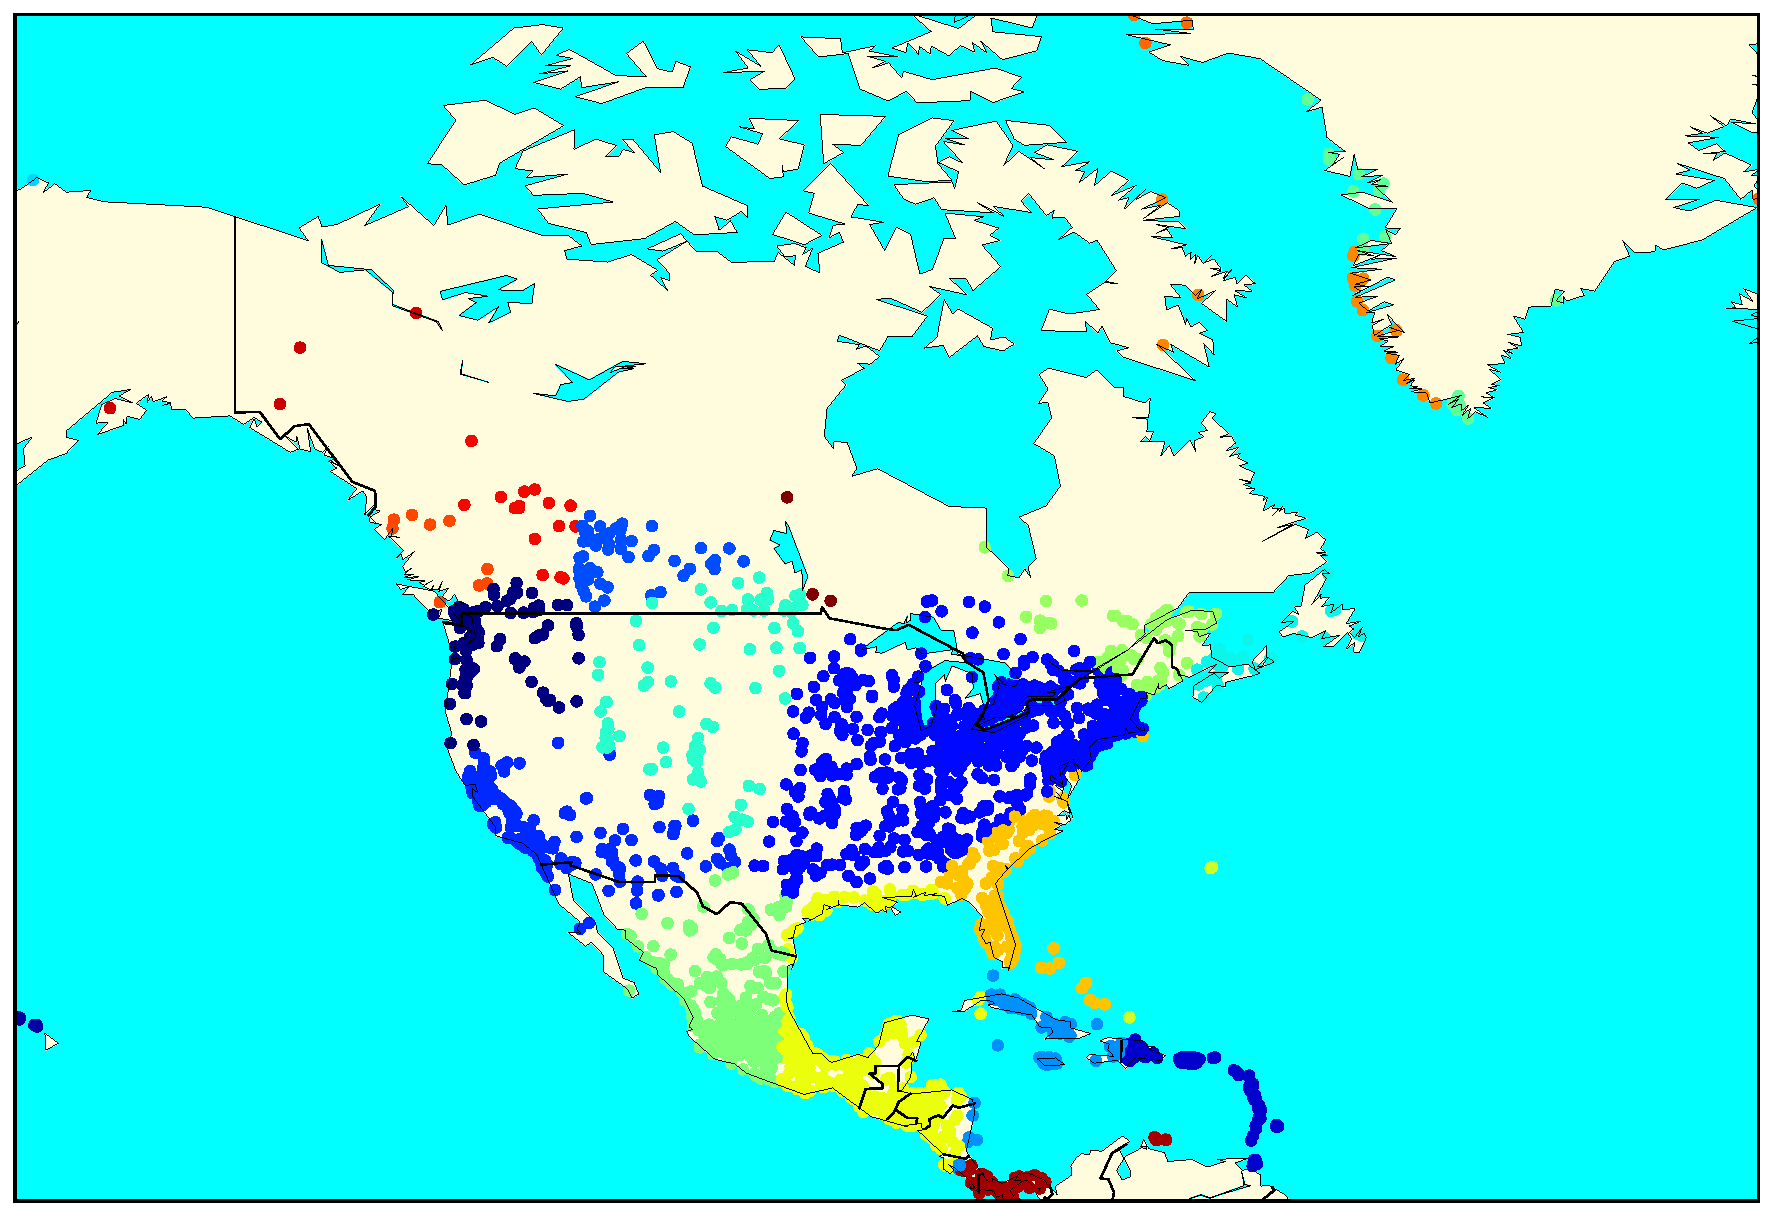
\includegraphics[width=8cm]{NA_k_means.pdf} &
				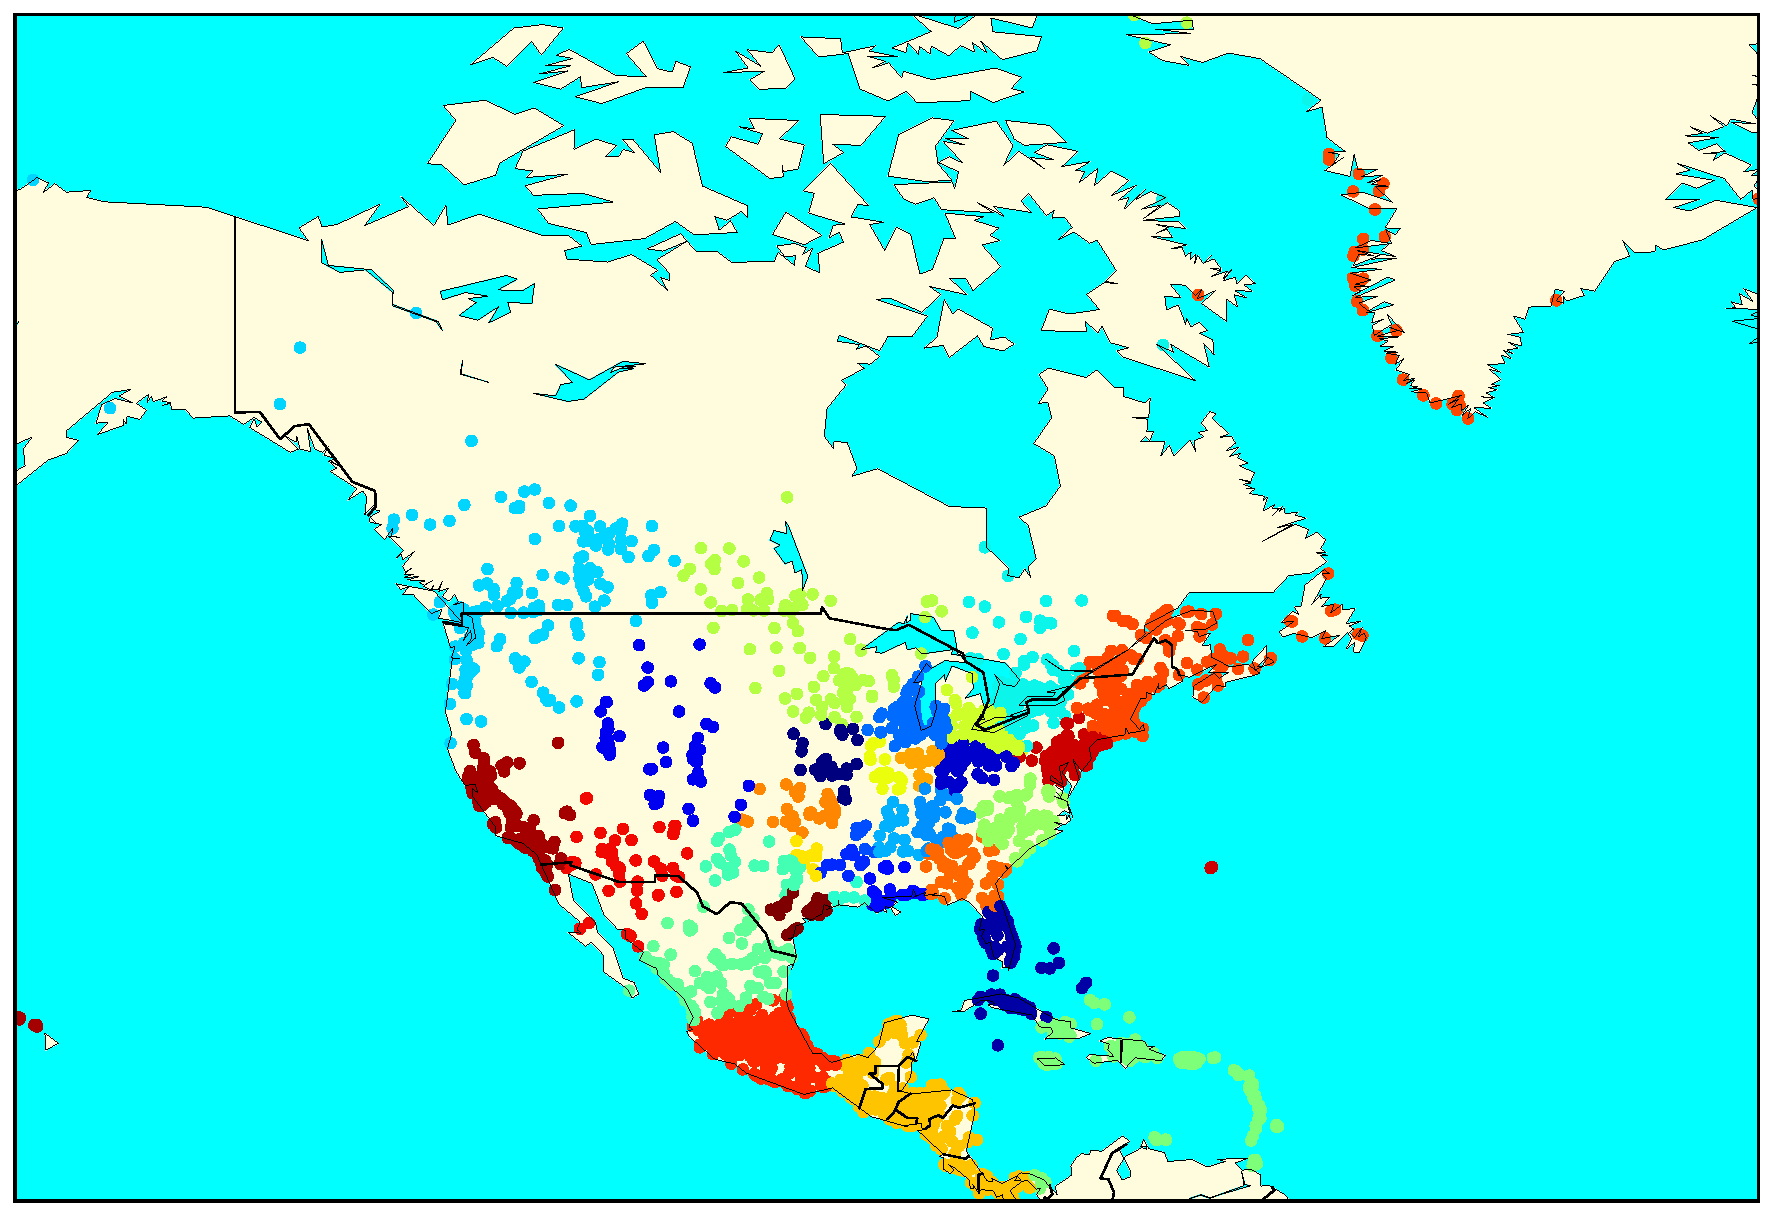
\includegraphics[width=8cm]{NA_k_medoids.pdf} \\
			\end{tabular}

			Южная Америка

			\begin{tabular}{c c}
				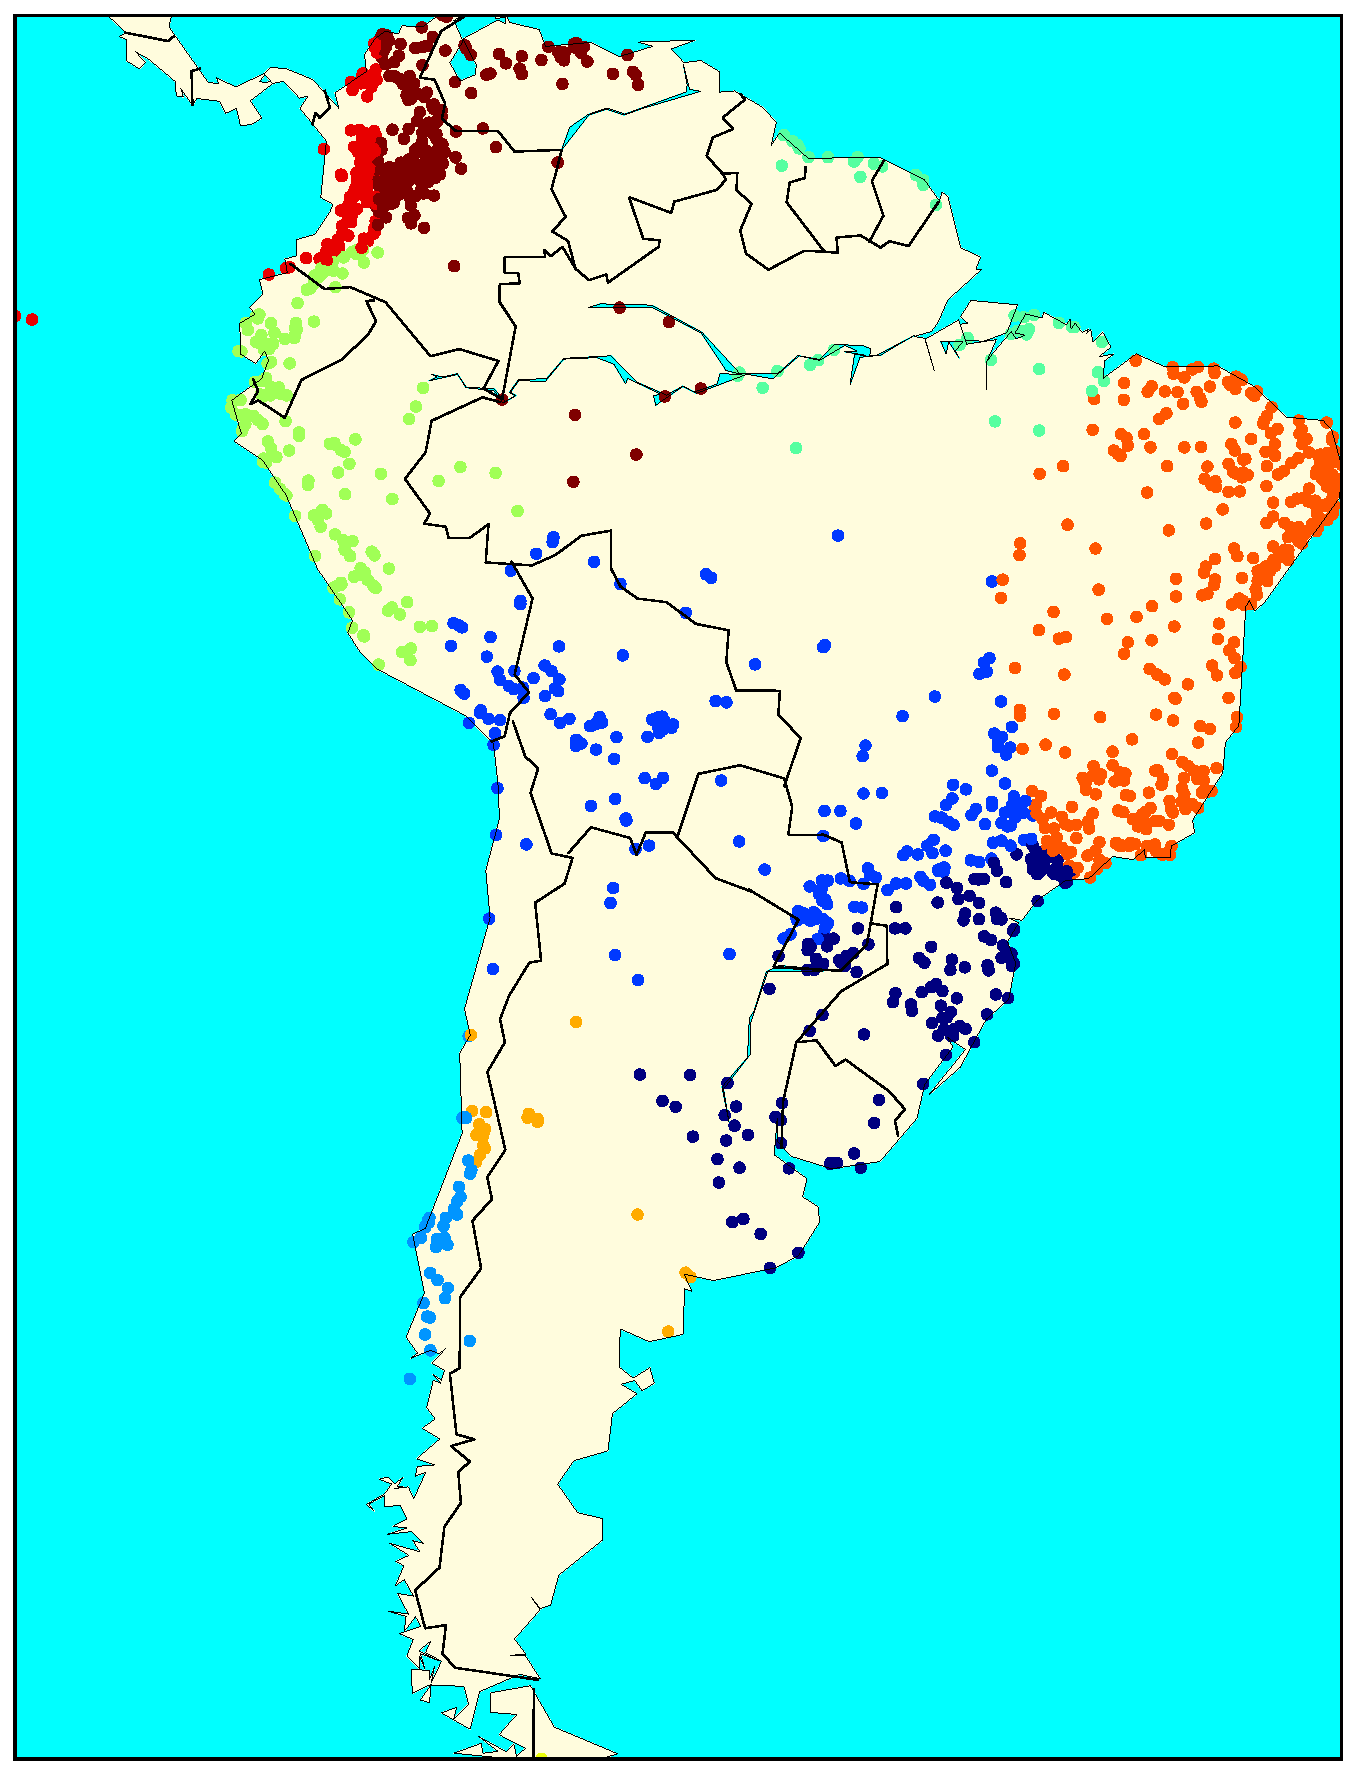
\includegraphics[width=8cm]{SA_k_means.pdf} &
				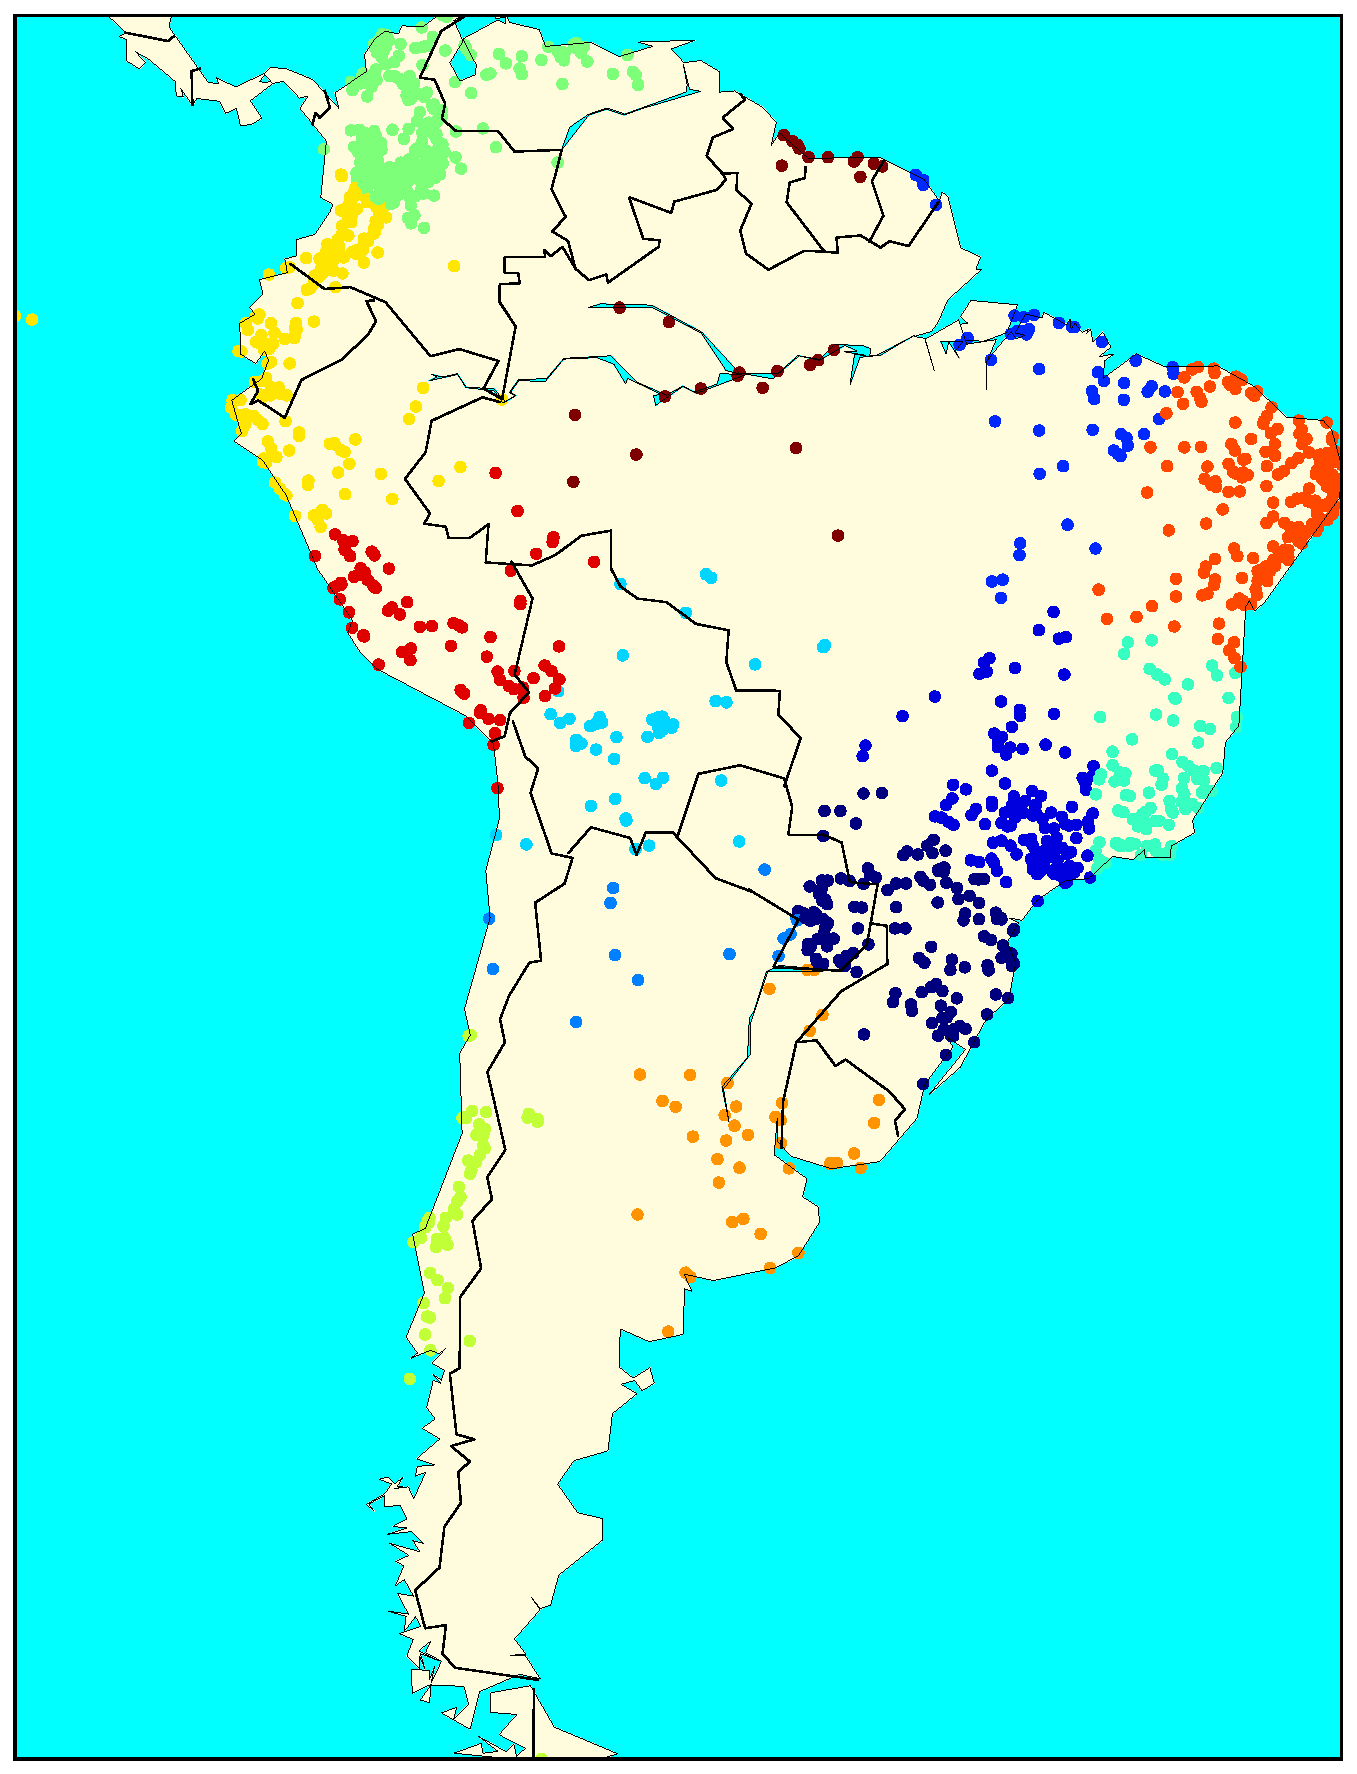
\includegraphics[width=8cm]{SA_k_medoids.pdf} \\
			\end{tabular}
			\end{center}

			\newpage
			\begin{center}
				И наконец на всем Мире:

				k-Means

				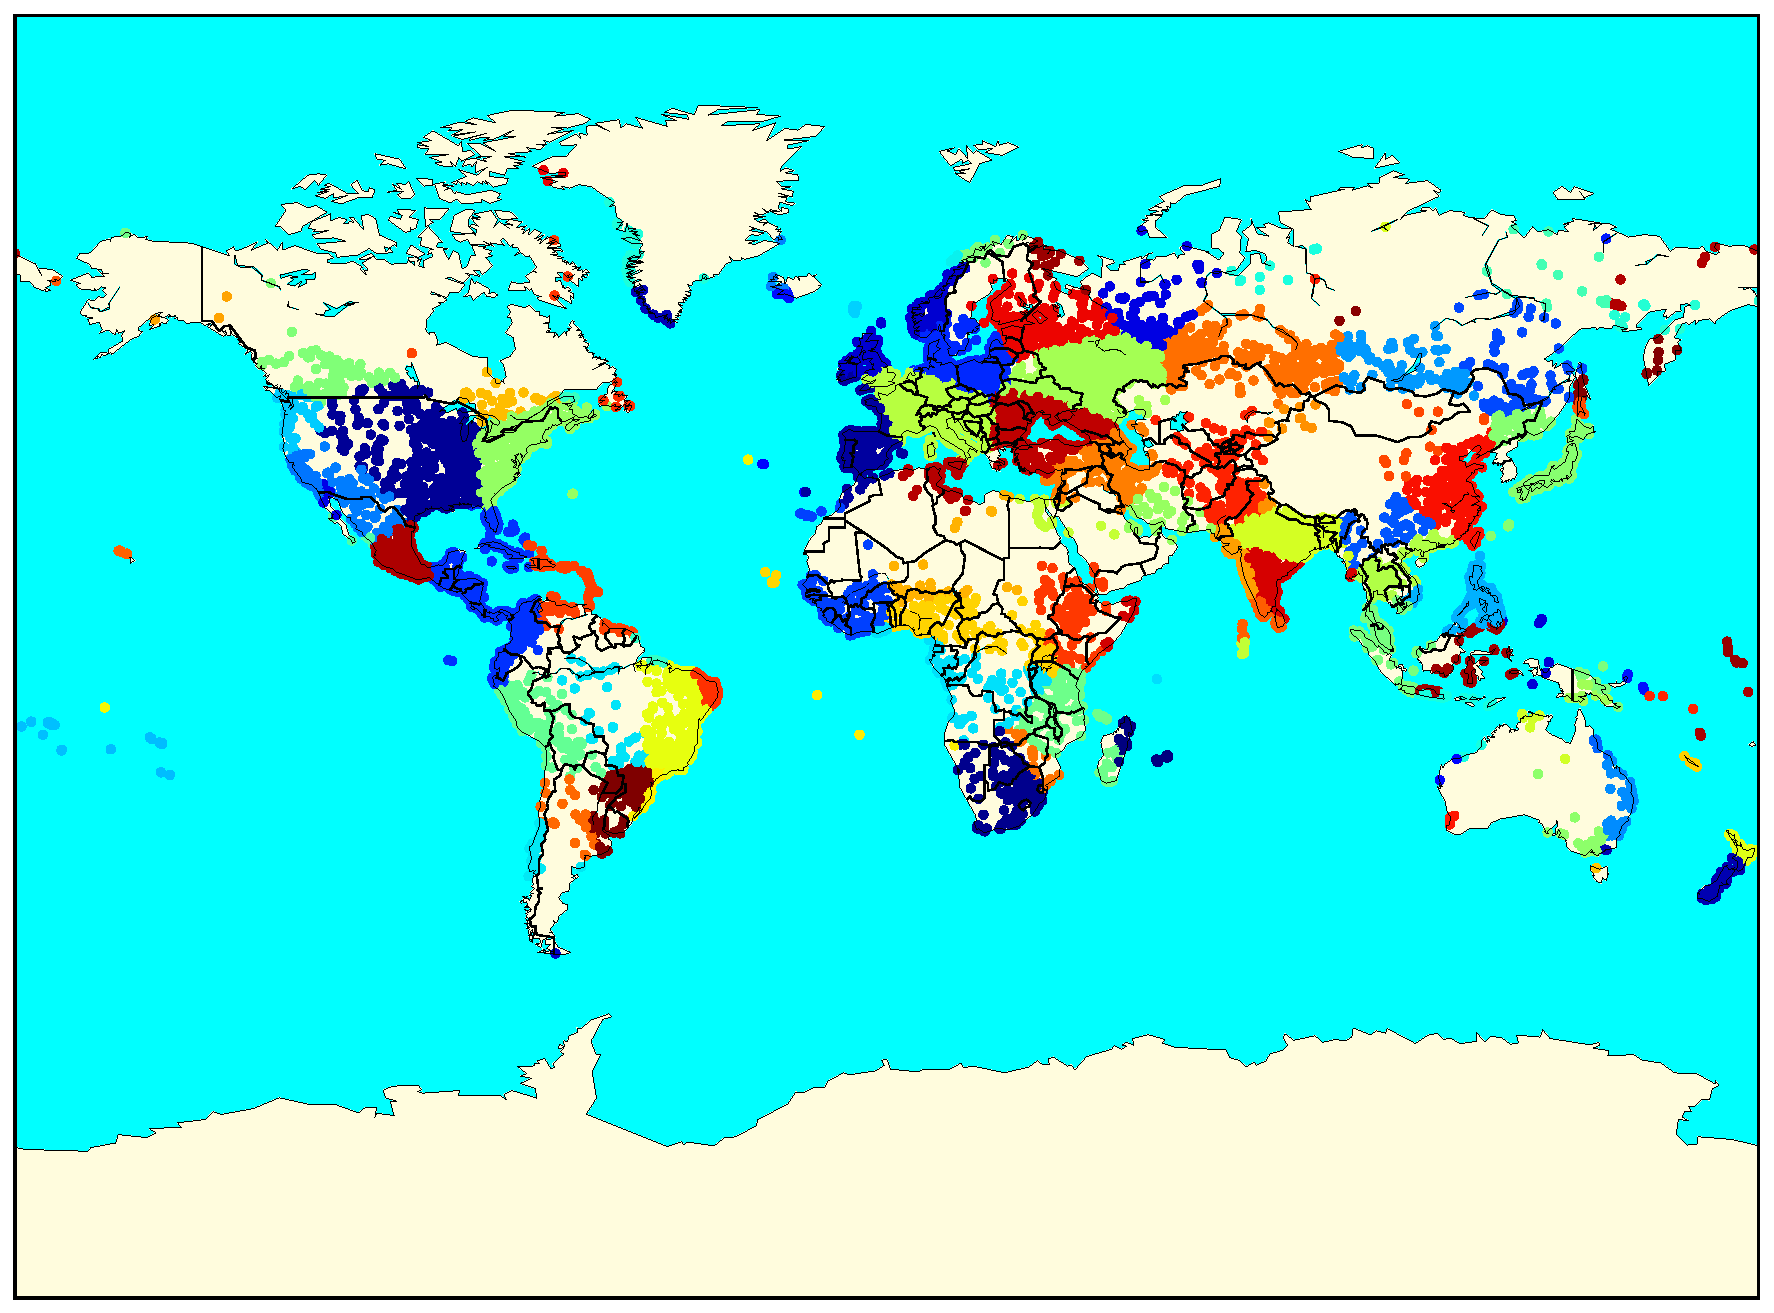
\includegraphics[width=15cm]{W_k_means.pdf}

				k-Medoids

				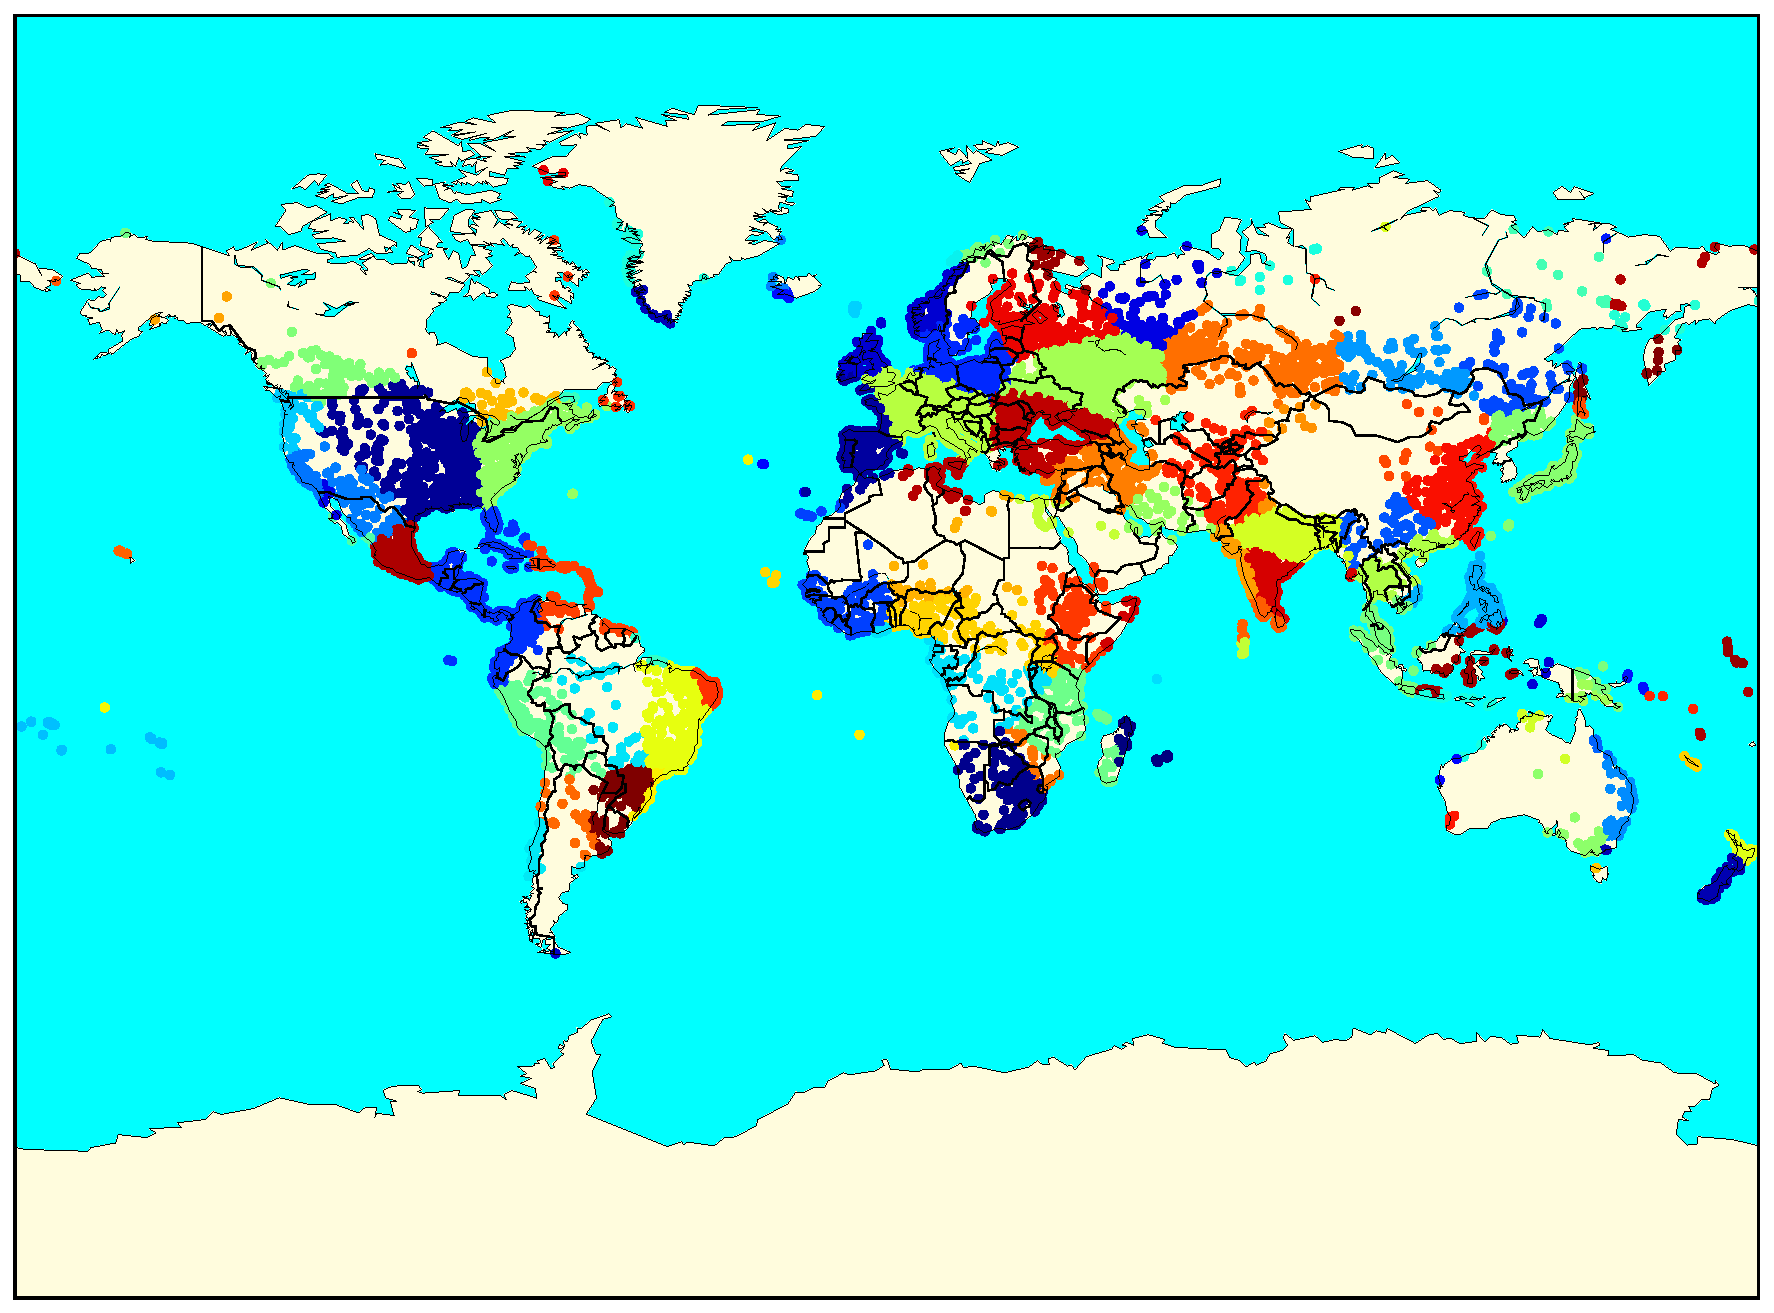
\includegraphics[width=15cm]{W_k_means.pdf}
			\end{center}


	\newpage
	\section{Заключение}
		В результате исследовательской работы выяснилось, что один и тот же код написанный на Python работает хуже, чем код напсанный на Cython и тем более на C++. Но при этом точность не пострадала. Все результаты можно видеть в пунктах~\ref{sssec:comp} и~\ref{sssec:test}.

		Для ускорения методов не применялось ничего заоблачного и в основном код не ускорялся. Для уменьшения вычислительных расходов радиус сферы брался равной единице. А для передачи данных в функцию на C++ использовался передача по адресу.

\end{document}
